% Chapter 3: α-stable distributions
% Statistics of Financial Markets -- Bachelor's programme, Bucharest University of Economic Studies
% GENERATED by latex/build_chapter3.py -- edit the generator, not this file.

\newcommand{\coursename}{Statistics of Financial Markets}
% Preambul comun SFM -- Statistica piețelor financiare / Statistics of Financial Markets (Beamer, 16:9)
% Același design ca MFM. Înainte de % Preambul comun SFM -- Statistica piețelor financiare / Statistics of Financial Markets (Beamer, 16:9)
% Același design ca MFM. Înainte de % Preambul comun SFM -- Statistica piețelor financiare / Statistics of Financial Markets (Beamer, 16:9)
% Același design ca MFM. Înainte de \input{../../latex/preamble} se definește
%   \newcommand{\coursename}{Statistics of Financial Markets}      (EN)
%   \newcommand{\coursename}{Statistica piețelor financiare}       (RO)  și  \def\sfmlang{ro}
% Fișierele .tex se află în EN/Courses, EN/Seminars, RO/Cursuri, RO/Seminarii (două niveluri sub rădăcină).
% Deck-urile sînt generate de latex/build_chapterN.py / build_seminarN.py (vezi latex/sfm_build.py).

\documentclass[9pt, aspectratio=169, t]{beamer}
\providecommand{\coursename}{Statistics of Financial Markets}

% Ensure content fits on slides
\setbeamersize{text margin left=8mm, text margin right=8mm}

%=============================================================================
% THEME AND STYLE CONFIGURATION
%=============================================================================
\usetheme{default}
% Using default theme for clean header/footer control

% Color Palette (matching Redispatch PDF)
\definecolor{MainBlue}{RGB}{26, 58, 110}
\definecolor{AccentBlue}{RGB}{26, 58, 110}
\definecolor{IDAred}{RGB}{205, 0, 0}
\definecolor{DarkGray}{RGB}{51, 51, 51}
\definecolor{MediumGray}{RGB}{128, 128, 128}
\definecolor{LightGray}{RGB}{248, 248, 248}
\definecolor{VeryLightGray}{RGB}{235, 235, 235}
\definecolor{KeynoteGray}{RGB}{218, 218, 218}
\definecolor{SectionGray}{RGB}{120, 120, 120}
\definecolor{FooterGray}{RGB}{100, 100, 100}
\definecolor{Crimson}{RGB}{220, 53, 69}
\definecolor{Forest}{RGB}{46, 125, 50}
\definecolor{Amber}{RGB}{181, 133, 63}
\definecolor{Orange}{RGB}{230, 126, 34}
\definecolor{Purple}{RGB}{142, 68, 173}

% Gradient background (exact Keynote 315° gradient: white to RGB 218,218,218)
\setbeamertemplate{background}{%
    \begin{tikzpicture}[remember picture, overlay]
        \shade[shading=axis, shading angle=315,
        top color=white, bottom color=KeynoteGray]
        (current page.south west) rectangle (current page.north east);
    \end{tikzpicture}%
}
% Fallback solid color for compatibility
\setbeamercolor{background canvas}{bg=}

\setbeamercolor{palette primary}{bg=MainBlue, fg=white}
\setbeamercolor{palette secondary}{bg=MainBlue!85, fg=white}
\setbeamercolor{palette tertiary}{bg=MainBlue!70, fg=white}
\setbeamercolor{structure}{fg=MainBlue}
\setbeamercolor{title}{fg=IDAred}
\setbeamercolor{frametitle}{fg=IDAred, bg=}
\setbeamercolor{block title}{bg=MainBlue, fg=white}
\setbeamercolor{block body}{bg=VeryLightGray, fg=DarkGray}
\setbeamercolor{block title alerted}{bg=Crimson, fg=white}
\setbeamercolor{block body alerted}{bg=Crimson!8, fg=DarkGray}
\setbeamercolor{block title example}{bg=Forest, fg=white}
\setbeamercolor{block body example}{bg=Forest!8, fg=DarkGray}
\setbeamercolor{item}{fg=MainBlue}

% Footer colors (override Madrid theme blue)
\setbeamercolor{author in head/foot}{fg=FooterGray, bg=}
\setbeamercolor{title in head/foot}{fg=FooterGray, bg=}
\setbeamercolor{date in head/foot}{fg=FooterGray, bg=}
\setbeamercolor{section in head/foot}{fg=FooterGray, bg=}
\setbeamercolor{subsection in head/foot}{fg=FooterGray, bg=}

% Bullet styles (apply everywhere including blocks)
\setbeamertemplate{itemize item}{\color{MainBlue}$\boxdot$}
\setbeamertemplate{itemize subitem}{\color{MainBlue}$\blacktriangleright$}
\setbeamertemplate{itemize subsubitem}{\color{MainBlue}\tiny$\bullet$}
\setbeamertemplate{itemize/enumerate body begin}{\normalsize}
\setbeamertemplate{itemize/enumerate subbody begin}{\normalsize}

% Item spacing - compact style
\setlength{\leftmargini}{10pt}       % Level 1: minimal indent
\setlength{\leftmarginii}{10pt}      % Level 2: minimal additional indent
% Compact list spacing (zero extra space before/after lists in blocks)
\makeatletter
\def\@listi{\leftmargin\leftmargini \topsep 0pt \parsep 0pt \itemsep 0pt}
\def\@listii{\leftmargin\leftmarginii \topsep 0pt \parsep 0pt \itemsep 0pt}
\makeatother

\setbeamertemplate{navigation symbols}{}

%=============================================================================
% CUSTOM HEADLINE
%=============================================================================
\setbeamertemplate{headline}{%
    \vskip10pt%
    \hbox to \paperwidth{%
        \hskip0.5cm%
        {\small\color{FooterGray}\renewcommand{\hyperlink}[2]{##2}\insertsectionhead}%
        \hfill%
        \textcolor{FooterGray}{\small\insertframenumber}%
        \hskip0.5cm%
    }%
    \vskip4pt%
    {\color{FooterGray}\hrule height 0.4pt}%
}

%=============================================================================
% CUSTOM FOOTER
%=============================================================================
\usepackage{fontawesome5}

\setbeamertemplate{footline}{%
    {\color{FooterGray}\hrule height 0.4pt}%
    \vskip4pt%
    \hbox to \paperwidth{%
        \hskip0.5cm%
        \textcolor{FooterGray}{\small\coursename}%
        \hfill%
        \raisebox{-0.1em}{%
            \begin{tikzpicture}[x=0.08em, y=0.08em, line width=0.4pt]
                \draw[FooterGray] (0,3) -- (1,4) -- (2,3.5) -- (3,5) -- (4,4) -- (5,6) -- (6,5.5) -- (7,4) -- (8,5) -- (9,7) -- (10,6) -- (11,5) -- (12,6.5) -- (13,8) -- (14,7) -- (15,6) -- (16,7.5) -- (17,9) -- (18,8) -- (19,7) -- (20,8.5) -- (21,10) -- (22,9) -- (23,8) -- (24,9.5);
            \end{tikzpicture}%
        }%
        \hskip0.5cm%
    }%
    \vskip6pt%
}

%=============================================================================
% PACKAGES
%=============================================================================
\usepackage[utf8]{inputenc}
\DeclareUnicodeCharacter{03B1}{\ensuremath{\alpha}}
\usepackage[T1]{fontenc}
\usepackage{amsmath, amssymb, amsthm}
\usepackage{mathtools}
\usepackage{bm}
\usepackage{tikz}
\usetikzlibrary{arrows.meta, positioning, shapes, calc, decorations.pathreplacing, shadings}
\usepackage{booktabs}
\usepackage{multirow}
\usepackage{array}
\usepackage{graphicx}
\usepackage{hyperref}
\usepackage{colortbl}
\usepackage{listings}
\lstset{language=Python, basicstyle=\ttfamily\scriptsize, keywordstyle=\color{MainBlue}\bfseries,
  commentstyle=\color{Forest}, stringstyle=\color{Crimson}, breaklines=true,
  frame=none, backgroundcolor=\color{VeryLightGray}, xleftmargin=2mm}
\hypersetup{colorlinks=true, linkcolor=MainBlue, urlcolor=MainBlue}
\graphicspath{{../../logos/}{../../charts/}{../../photos/}}
\usepackage{xcolor}
\hfuzz=2pt  % Suppress tiny overfull warnings (<2pt)
\vfuzz=2pt  % Suppress tiny vertical overfull warnings (<2pt)

%=============================================================================
% QUANTLET COMMANDS
%   \quantlet{<displayed name>}{<url>}       (generic, compatible with the older SFM decks)
%   \sfmquantlet{Ch_05}{SFM_ch5_garch}       -> https://github.com/danpele/SFM/tree/main/Quantlets/Ch_05/SFM_ch5_garch
%   \qlurl{<folder>} is defined per chapter by the generator (Quantlets/Ch_NN/<folder>)
%=============================================================================
\newcommand{\sfmrepo}{https://github.com/danpele/SFM}
\newcommand{\sfmqlbase}{https://github.com/danpele/SFM/tree/main/Quantlets}
\newcommand{\quantlet}[2]{%
    \hfill\href{#2}{%
        \raisebox{-0.15em}{
\includegraphics[height=0.7em]{ql_logo.png}}%
        \textcolor{MainBlue}{\tiny\ #1}%
    }%
}
\newcommand{\sfmquantlet}[2]{\quantlet{\detokenize{#2}}{\sfmqlbase/#1/#2}}

%=============================================================================
% NOTEBOOKS (Google Colab)
%   \colaburl{notebooks/EN/chapter5_seminar_notebook.ipynb} -> the Colab link of a file in the SFM repo
%   \nb: the chapter notebook (each seminar deck redefines it with \renewcommand)
%=============================================================================
\newcommand{\colaburl}[1]{https://colab.research.google.com/github/danpele/SFM/blob/main/#1}
\newcommand{\nb}{https://colab.research.google.com/github/danpele/SFM/tree/main/notebooks/EN}
\newcommand{\nbname}{notebooks/EN}

%=============================================================================
% SLIDE HELPERS (used by the generators; the same as in MFM)
%=============================================================================
% local font size for list bodies (the preamble forces \normalsize)
\newcommand{\itemsize}[1]{\setbeamertemplate{itemize/enumerate body begin}{#1}\setbeamertemplate{itemize/enumerate subbody begin}{#1}}
\newcommand{\intitle}[1]{{\hypersetup{urlcolor=white}#1}}   % white links inside coloured title bars
\newcommand{\imgcap}[1]{{\scriptsize #1}\\[0.5mm]}          % caption under a photo
\newcommand{\imgcredit}[2]{{\tiny\color{FooterGray}\href{#1}{#2}}}   % image credit: source URL, author/licence
\newcommand{\aiprompt}[1]{{\ttfamily\color{MainBlue}#1}}     % a prompt to an AI assistant

%=============================================================================
% SEMINARS: student version by default; the instructor wrapper *_solutions.tex sets \solutionstrue
%=============================================================================
\makeatletter\@ifundefined{ifsolutions}{\expandafter\newif\csname ifsolutions\endcsname}{}\makeatother
\newcommand{\solonly}[1]{\ifsolutions #1\fi}
\newcommand{\propsub}{\ifsolutions\else\framesubtitle{\ifdefined\sfmlang Rezolvarea se discută la seminar\else Solution discussed in class\fi}\fi}

%=============================================================================
% APPENDIX AND CHAPTER LINKS (latex/appendix_links.py writes the calls; it also re-declares these
% macros before \begin{document}, so the decks compile with or without this preamble block)
%=============================================================================
\providecommand{\sfmapplink}[3]{\hypertarget{#2}{}\hyperlink{#1}{\beamergotobutton{#3}}}
\providecommand{\sfmappback}[2]{\begin{tikzpicture}[remember picture,overlay]\node[anchor=south east] at ([xshift=-3mm,yshift=7mm]current page.south east){\hyperlink{#1}{\beamerreturnbutton{#2}}};\end{tikzpicture}}
\providecommand{\sfmchlink}[2]{\href{#1}{#2}}
\providecommand{\sfmchlinkt}[2]{\href{#1}{\usebeamercolor[fg]{frametitle}#2}}

%=============================================================================
% QUANTINAR COMMAND: link către un curs Quantinar (subiecte avansate)
%=============================================================================
\newcommand{\quantinar}[2]{%
    \href{#2}{%
        \raisebox{-0.15em}{
\includegraphics[height=0.8em]{qr_logo.png}}%
        \textcolor{MainBlue}{\scriptsize\ #1}%
    }%
}

%=============================================================================
% CUSTOM TITLE PAGE
%=============================================================================
\defbeamertemplate*{title page}{hybrid}[1][]
{
    \vspace{0.2cm}
    % Logos row - top header (with clickable links)
    \begin{center}
        \href{https://www.ase.ro}{
\includegraphics[height=1.0cm]{ase_logo.png}}\hspace{0.3cm}%
        \href{https://theida.net}{
\includegraphics[height=1.0cm]{ida_logo.png}}\hspace{0.3cm}%
        \href{https://blockchain-research-center.com}{
\includegraphics[height=1.0cm]{brc_logo.png}}\hspace{0.3cm}%
        \href{https://www.ai4efin.ase.ro}{
\includegraphics[height=1.0cm]{ai4efin_logo.png}}\hspace{0.3cm}%
        \href{https://ipe.ro/new}{
\includegraphics[height=1.0cm]{acad_logo.png}}\hspace{0.3cm}%
        \href{https://www.digital-finance-msca.com}{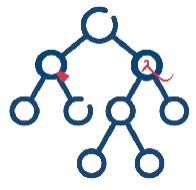
\includegraphics[height=1.0cm]{msca_logo.png}}%
    \end{center}

    \vspace{0.6cm}

    % Main title with Q logos on sides (with clickable links)
    \begin{center}
        \begin{minipage}{0.1\textwidth}
            \centering
            \href{https://quantlet.com}{
\includegraphics[height=1.1cm]{ql_logo.png}}
        \end{minipage}%
        \begin{minipage}{0.78\textwidth}
            \centering
            {\LARGE\bfseries\usebeamercolor[fg]{title}\inserttitle}

            \vspace{0.3cm}

            {\usebeamerfont{subtitle}\usebeamercolor[fg]{title}\insertsubtitle}
        \end{minipage}%
        \begin{minipage}{0.1\textwidth}
            \centering
            \href{https://quantinar.com}{
\includegraphics[height=1.1cm]{qr_logo.png}}
        \end{minipage}
    \end{center}

    \vspace{0.6cm}

    % Authors (left aligned)
    \hspace{0.5cm}{\usebeamerfont{author}\insertauthor}

    \vspace{0.3cm}

    % Institute/Affiliations (left aligned)
    \hspace{0.5cm}\begin{minipage}[t]{0.9\textwidth}
        \raggedright\small\insertinstitute
    \end{minipage}
}

%=============================================================================
% THEOREM ENVIRONMENTS
%=============================================================================
\theoremstyle{definition}
\setbeamertemplate{theorems}[numbered]
\ifdefined\sfmlang
\newtheorem{defn}{Definiție}
\newtheorem{thm}{Teoremă}
\newtheorem{prop}{Propoziție}
\newtheorem{rmk}{Observație}
\else
\newtheorem{defn}{Definition}
\newtheorem{thm}{Theorem}
\newtheorem{prop}{Proposition}
\newtheorem{rmk}{Remark}
\fi

%=============================================================================
% CENTRED MINIPAGE (no extra vertical space)
%=============================================================================
\newenvironment{cminipage}[1]{%
    \par\noindent\hfill\begin{minipage}{#1}\ignorespaces
}{%
    \end{minipage}\hfill\null\par
}

%=============================================================================
% CUSTOM COMMANDS
%=============================================================================
\newcommand{\E}{\mathbb{E}}
\newcommand{\Var}{\text{Var}}
\newcommand{\Cov}{\text{Cov}}
\newcommand{\Corr}{\text{Corr}}
\newcommand{\R}{\mathbb{R}}
\newcommand{\N}{\mathbb{N}}
\newcommand{\Z}{\mathbb{Z}}
\newcommand{\B}{\mathbf{B}}
\newcommand{\imark}{\textcolor{MainBlue}{\textbullet}}
\newcommand{\RMSE}{\text{RMSE}}
\newcommand{\MAE}{\text{MAE}}
\newcommand{\MAPE}{\text{MAPE}}

 se definește
%   \newcommand{\coursename}{Statistics of Financial Markets}      (EN)
%   \newcommand{\coursename}{Statistica piețelor financiare}       (RO)  și  \def\sfmlang{ro}
% Fișierele .tex se află în EN/Courses, EN/Seminars, RO/Cursuri, RO/Seminarii (două niveluri sub rădăcină).
% Deck-urile sînt generate de latex/build_chapterN.py / build_seminarN.py (vezi latex/sfm_build.py).

\documentclass[9pt, aspectratio=169, t]{beamer}
\providecommand{\coursename}{Statistics of Financial Markets}

% Ensure content fits on slides
\setbeamersize{text margin left=8mm, text margin right=8mm}

%=============================================================================
% THEME AND STYLE CONFIGURATION
%=============================================================================
\usetheme{default}
% Using default theme for clean header/footer control

% Color Palette (matching Redispatch PDF)
\definecolor{MainBlue}{RGB}{26, 58, 110}
\definecolor{AccentBlue}{RGB}{26, 58, 110}
\definecolor{IDAred}{RGB}{205, 0, 0}
\definecolor{DarkGray}{RGB}{51, 51, 51}
\definecolor{MediumGray}{RGB}{128, 128, 128}
\definecolor{LightGray}{RGB}{248, 248, 248}
\definecolor{VeryLightGray}{RGB}{235, 235, 235}
\definecolor{KeynoteGray}{RGB}{218, 218, 218}
\definecolor{SectionGray}{RGB}{120, 120, 120}
\definecolor{FooterGray}{RGB}{100, 100, 100}
\definecolor{Crimson}{RGB}{220, 53, 69}
\definecolor{Forest}{RGB}{46, 125, 50}
\definecolor{Amber}{RGB}{181, 133, 63}
\definecolor{Orange}{RGB}{230, 126, 34}
\definecolor{Purple}{RGB}{142, 68, 173}

% Gradient background (exact Keynote 315° gradient: white to RGB 218,218,218)
\setbeamertemplate{background}{%
    \begin{tikzpicture}[remember picture, overlay]
        \shade[shading=axis, shading angle=315,
        top color=white, bottom color=KeynoteGray]
        (current page.south west) rectangle (current page.north east);
    \end{tikzpicture}%
}
% Fallback solid color for compatibility
\setbeamercolor{background canvas}{bg=}

\setbeamercolor{palette primary}{bg=MainBlue, fg=white}
\setbeamercolor{palette secondary}{bg=MainBlue!85, fg=white}
\setbeamercolor{palette tertiary}{bg=MainBlue!70, fg=white}
\setbeamercolor{structure}{fg=MainBlue}
\setbeamercolor{title}{fg=IDAred}
\setbeamercolor{frametitle}{fg=IDAred, bg=}
\setbeamercolor{block title}{bg=MainBlue, fg=white}
\setbeamercolor{block body}{bg=VeryLightGray, fg=DarkGray}
\setbeamercolor{block title alerted}{bg=Crimson, fg=white}
\setbeamercolor{block body alerted}{bg=Crimson!8, fg=DarkGray}
\setbeamercolor{block title example}{bg=Forest, fg=white}
\setbeamercolor{block body example}{bg=Forest!8, fg=DarkGray}
\setbeamercolor{item}{fg=MainBlue}

% Footer colors (override Madrid theme blue)
\setbeamercolor{author in head/foot}{fg=FooterGray, bg=}
\setbeamercolor{title in head/foot}{fg=FooterGray, bg=}
\setbeamercolor{date in head/foot}{fg=FooterGray, bg=}
\setbeamercolor{section in head/foot}{fg=FooterGray, bg=}
\setbeamercolor{subsection in head/foot}{fg=FooterGray, bg=}

% Bullet styles (apply everywhere including blocks)
\setbeamertemplate{itemize item}{\color{MainBlue}$\boxdot$}
\setbeamertemplate{itemize subitem}{\color{MainBlue}$\blacktriangleright$}
\setbeamertemplate{itemize subsubitem}{\color{MainBlue}\tiny$\bullet$}
\setbeamertemplate{itemize/enumerate body begin}{\normalsize}
\setbeamertemplate{itemize/enumerate subbody begin}{\normalsize}

% Item spacing - compact style
\setlength{\leftmargini}{10pt}       % Level 1: minimal indent
\setlength{\leftmarginii}{10pt}      % Level 2: minimal additional indent
% Compact list spacing (zero extra space before/after lists in blocks)
\makeatletter
\def\@listi{\leftmargin\leftmargini \topsep 0pt \parsep 0pt \itemsep 0pt}
\def\@listii{\leftmargin\leftmarginii \topsep 0pt \parsep 0pt \itemsep 0pt}
\makeatother

\setbeamertemplate{navigation symbols}{}

%=============================================================================
% CUSTOM HEADLINE
%=============================================================================
\setbeamertemplate{headline}{%
    \vskip10pt%
    \hbox to \paperwidth{%
        \hskip0.5cm%
        {\small\color{FooterGray}\renewcommand{\hyperlink}[2]{##2}\insertsectionhead}%
        \hfill%
        \textcolor{FooterGray}{\small\insertframenumber}%
        \hskip0.5cm%
    }%
    \vskip4pt%
    {\color{FooterGray}\hrule height 0.4pt}%
}

%=============================================================================
% CUSTOM FOOTER
%=============================================================================
\usepackage{fontawesome5}

\setbeamertemplate{footline}{%
    {\color{FooterGray}\hrule height 0.4pt}%
    \vskip4pt%
    \hbox to \paperwidth{%
        \hskip0.5cm%
        \textcolor{FooterGray}{\small\coursename}%
        \hfill%
        \raisebox{-0.1em}{%
            \begin{tikzpicture}[x=0.08em, y=0.08em, line width=0.4pt]
                \draw[FooterGray] (0,3) -- (1,4) -- (2,3.5) -- (3,5) -- (4,4) -- (5,6) -- (6,5.5) -- (7,4) -- (8,5) -- (9,7) -- (10,6) -- (11,5) -- (12,6.5) -- (13,8) -- (14,7) -- (15,6) -- (16,7.5) -- (17,9) -- (18,8) -- (19,7) -- (20,8.5) -- (21,10) -- (22,9) -- (23,8) -- (24,9.5);
            \end{tikzpicture}%
        }%
        \hskip0.5cm%
    }%
    \vskip6pt%
}

%=============================================================================
% PACKAGES
%=============================================================================
\usepackage[utf8]{inputenc}
\DeclareUnicodeCharacter{03B1}{\ensuremath{\alpha}}
\usepackage[T1]{fontenc}
\usepackage{amsmath, amssymb, amsthm}
\usepackage{mathtools}
\usepackage{bm}
\usepackage{tikz}
\usetikzlibrary{arrows.meta, positioning, shapes, calc, decorations.pathreplacing, shadings}
\usepackage{booktabs}
\usepackage{multirow}
\usepackage{array}
\usepackage{graphicx}
\usepackage{hyperref}
\usepackage{colortbl}
\usepackage{listings}
\lstset{language=Python, basicstyle=\ttfamily\scriptsize, keywordstyle=\color{MainBlue}\bfseries,
  commentstyle=\color{Forest}, stringstyle=\color{Crimson}, breaklines=true,
  frame=none, backgroundcolor=\color{VeryLightGray}, xleftmargin=2mm}
\hypersetup{colorlinks=true, linkcolor=MainBlue, urlcolor=MainBlue}
\graphicspath{{../../logos/}{../../charts/}{../../photos/}}
\usepackage{xcolor}
\hfuzz=2pt  % Suppress tiny overfull warnings (<2pt)
\vfuzz=2pt  % Suppress tiny vertical overfull warnings (<2pt)

%=============================================================================
% QUANTLET COMMANDS
%   \quantlet{<displayed name>}{<url>}       (generic, compatible with the older SFM decks)
%   \sfmquantlet{Ch_05}{SFM_ch5_garch}       -> https://github.com/danpele/SFM/tree/main/Quantlets/Ch_05/SFM_ch5_garch
%   \qlurl{<folder>} is defined per chapter by the generator (Quantlets/Ch_NN/<folder>)
%=============================================================================
\newcommand{\sfmrepo}{https://github.com/danpele/SFM}
\newcommand{\sfmqlbase}{https://github.com/danpele/SFM/tree/main/Quantlets}
\newcommand{\quantlet}[2]{%
    \hfill\href{#2}{%
        \raisebox{-0.15em}{
\includegraphics[height=0.7em]{ql_logo.png}}%
        \textcolor{MainBlue}{\tiny\ #1}%
    }%
}
\newcommand{\sfmquantlet}[2]{\quantlet{\detokenize{#2}}{\sfmqlbase/#1/#2}}

%=============================================================================
% NOTEBOOKS (Google Colab)
%   \colaburl{notebooks/EN/chapter5_seminar_notebook.ipynb} -> the Colab link of a file in the SFM repo
%   \nb: the chapter notebook (each seminar deck redefines it with \renewcommand)
%=============================================================================
\newcommand{\colaburl}[1]{https://colab.research.google.com/github/danpele/SFM/blob/main/#1}
\newcommand{\nb}{https://colab.research.google.com/github/danpele/SFM/tree/main/notebooks/EN}
\newcommand{\nbname}{notebooks/EN}

%=============================================================================
% SLIDE HELPERS (used by the generators; the same as in MFM)
%=============================================================================
% local font size for list bodies (the preamble forces \normalsize)
\newcommand{\itemsize}[1]{\setbeamertemplate{itemize/enumerate body begin}{#1}\setbeamertemplate{itemize/enumerate subbody begin}{#1}}
\newcommand{\intitle}[1]{{\hypersetup{urlcolor=white}#1}}   % white links inside coloured title bars
\newcommand{\imgcap}[1]{{\scriptsize #1}\\[0.5mm]}          % caption under a photo
\newcommand{\imgcredit}[2]{{\tiny\color{FooterGray}\href{#1}{#2}}}   % image credit: source URL, author/licence
\newcommand{\aiprompt}[1]{{\ttfamily\color{MainBlue}#1}}     % a prompt to an AI assistant

%=============================================================================
% SEMINARS: student version by default; the instructor wrapper *_solutions.tex sets \solutionstrue
%=============================================================================
\makeatletter\@ifundefined{ifsolutions}{\expandafter\newif\csname ifsolutions\endcsname}{}\makeatother
\newcommand{\solonly}[1]{\ifsolutions #1\fi}
\newcommand{\propsub}{\ifsolutions\else\framesubtitle{\ifdefined\sfmlang Rezolvarea se discută la seminar\else Solution discussed in class\fi}\fi}

%=============================================================================
% APPENDIX AND CHAPTER LINKS (latex/appendix_links.py writes the calls; it also re-declares these
% macros before \begin{document}, so the decks compile with or without this preamble block)
%=============================================================================
\providecommand{\sfmapplink}[3]{\hypertarget{#2}{}\hyperlink{#1}{\beamergotobutton{#3}}}
\providecommand{\sfmappback}[2]{\begin{tikzpicture}[remember picture,overlay]\node[anchor=south east] at ([xshift=-3mm,yshift=7mm]current page.south east){\hyperlink{#1}{\beamerreturnbutton{#2}}};\end{tikzpicture}}
\providecommand{\sfmchlink}[2]{\href{#1}{#2}}
\providecommand{\sfmchlinkt}[2]{\href{#1}{\usebeamercolor[fg]{frametitle}#2}}

%=============================================================================
% QUANTINAR COMMAND: link către un curs Quantinar (subiecte avansate)
%=============================================================================
\newcommand{\quantinar}[2]{%
    \href{#2}{%
        \raisebox{-0.15em}{
\includegraphics[height=0.8em]{qr_logo.png}}%
        \textcolor{MainBlue}{\scriptsize\ #1}%
    }%
}

%=============================================================================
% CUSTOM TITLE PAGE
%=============================================================================
\defbeamertemplate*{title page}{hybrid}[1][]
{
    \vspace{0.2cm}
    % Logos row - top header (with clickable links)
    \begin{center}
        \href{https://www.ase.ro}{
\includegraphics[height=1.0cm]{ase_logo.png}}\hspace{0.3cm}%
        \href{https://theida.net}{
\includegraphics[height=1.0cm]{ida_logo.png}}\hspace{0.3cm}%
        \href{https://blockchain-research-center.com}{
\includegraphics[height=1.0cm]{brc_logo.png}}\hspace{0.3cm}%
        \href{https://www.ai4efin.ase.ro}{
\includegraphics[height=1.0cm]{ai4efin_logo.png}}\hspace{0.3cm}%
        \href{https://ipe.ro/new}{
\includegraphics[height=1.0cm]{acad_logo.png}}\hspace{0.3cm}%
        \href{https://www.digital-finance-msca.com}{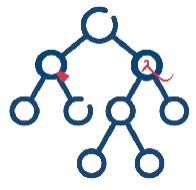
\includegraphics[height=1.0cm]{msca_logo.png}}%
    \end{center}

    \vspace{0.6cm}

    % Main title with Q logos on sides (with clickable links)
    \begin{center}
        \begin{minipage}{0.1\textwidth}
            \centering
            \href{https://quantlet.com}{
\includegraphics[height=1.1cm]{ql_logo.png}}
        \end{minipage}%
        \begin{minipage}{0.78\textwidth}
            \centering
            {\LARGE\bfseries\usebeamercolor[fg]{title}\inserttitle}

            \vspace{0.3cm}

            {\usebeamerfont{subtitle}\usebeamercolor[fg]{title}\insertsubtitle}
        \end{minipage}%
        \begin{minipage}{0.1\textwidth}
            \centering
            \href{https://quantinar.com}{
\includegraphics[height=1.1cm]{qr_logo.png}}
        \end{minipage}
    \end{center}

    \vspace{0.6cm}

    % Authors (left aligned)
    \hspace{0.5cm}{\usebeamerfont{author}\insertauthor}

    \vspace{0.3cm}

    % Institute/Affiliations (left aligned)
    \hspace{0.5cm}\begin{minipage}[t]{0.9\textwidth}
        \raggedright\small\insertinstitute
    \end{minipage}
}

%=============================================================================
% THEOREM ENVIRONMENTS
%=============================================================================
\theoremstyle{definition}
\setbeamertemplate{theorems}[numbered]
\ifdefined\sfmlang
\newtheorem{defn}{Definiție}
\newtheorem{thm}{Teoremă}
\newtheorem{prop}{Propoziție}
\newtheorem{rmk}{Observație}
\else
\newtheorem{defn}{Definition}
\newtheorem{thm}{Theorem}
\newtheorem{prop}{Proposition}
\newtheorem{rmk}{Remark}
\fi

%=============================================================================
% CENTRED MINIPAGE (no extra vertical space)
%=============================================================================
\newenvironment{cminipage}[1]{%
    \par\noindent\hfill\begin{minipage}{#1}\ignorespaces
}{%
    \end{minipage}\hfill\null\par
}

%=============================================================================
% CUSTOM COMMANDS
%=============================================================================
\newcommand{\E}{\mathbb{E}}
\newcommand{\Var}{\text{Var}}
\newcommand{\Cov}{\text{Cov}}
\newcommand{\Corr}{\text{Corr}}
\newcommand{\R}{\mathbb{R}}
\newcommand{\N}{\mathbb{N}}
\newcommand{\Z}{\mathbb{Z}}
\newcommand{\B}{\mathbf{B}}
\newcommand{\imark}{\textcolor{MainBlue}{\textbullet}}
\newcommand{\RMSE}{\text{RMSE}}
\newcommand{\MAE}{\text{MAE}}
\newcommand{\MAPE}{\text{MAPE}}

 se definește
%   \newcommand{\coursename}{Statistics of Financial Markets}      (EN)
%   \newcommand{\coursename}{Statistica piețelor financiare}       (RO)  și  \def\sfmlang{ro}
% Fișierele .tex se află în EN/Courses, EN/Seminars, RO/Cursuri, RO/Seminarii (două niveluri sub rădăcină).
% Deck-urile sînt generate de latex/build_chapterN.py / build_seminarN.py (vezi latex/sfm_build.py).

\documentclass[9pt, aspectratio=169, t]{beamer}
\providecommand{\coursename}{Statistics of Financial Markets}

% Ensure content fits on slides
\setbeamersize{text margin left=8mm, text margin right=8mm}

%=============================================================================
% THEME AND STYLE CONFIGURATION
%=============================================================================
\usetheme{default}
% Using default theme for clean header/footer control

% Color Palette (matching Redispatch PDF)
\definecolor{MainBlue}{RGB}{26, 58, 110}
\definecolor{AccentBlue}{RGB}{26, 58, 110}
\definecolor{IDAred}{RGB}{205, 0, 0}
\definecolor{DarkGray}{RGB}{51, 51, 51}
\definecolor{MediumGray}{RGB}{128, 128, 128}
\definecolor{LightGray}{RGB}{248, 248, 248}
\definecolor{VeryLightGray}{RGB}{235, 235, 235}
\definecolor{KeynoteGray}{RGB}{218, 218, 218}
\definecolor{SectionGray}{RGB}{120, 120, 120}
\definecolor{FooterGray}{RGB}{100, 100, 100}
\definecolor{Crimson}{RGB}{220, 53, 69}
\definecolor{Forest}{RGB}{46, 125, 50}
\definecolor{Amber}{RGB}{181, 133, 63}
\definecolor{Orange}{RGB}{230, 126, 34}
\definecolor{Purple}{RGB}{142, 68, 173}

% Gradient background (exact Keynote 315° gradient: white to RGB 218,218,218)
\setbeamertemplate{background}{%
    \begin{tikzpicture}[remember picture, overlay]
        \shade[shading=axis, shading angle=315,
        top color=white, bottom color=KeynoteGray]
        (current page.south west) rectangle (current page.north east);
    \end{tikzpicture}%
}
% Fallback solid color for compatibility
\setbeamercolor{background canvas}{bg=}

\setbeamercolor{palette primary}{bg=MainBlue, fg=white}
\setbeamercolor{palette secondary}{bg=MainBlue!85, fg=white}
\setbeamercolor{palette tertiary}{bg=MainBlue!70, fg=white}
\setbeamercolor{structure}{fg=MainBlue}
\setbeamercolor{title}{fg=IDAred}
\setbeamercolor{frametitle}{fg=IDAred, bg=}
\setbeamercolor{block title}{bg=MainBlue, fg=white}
\setbeamercolor{block body}{bg=VeryLightGray, fg=DarkGray}
\setbeamercolor{block title alerted}{bg=Crimson, fg=white}
\setbeamercolor{block body alerted}{bg=Crimson!8, fg=DarkGray}
\setbeamercolor{block title example}{bg=Forest, fg=white}
\setbeamercolor{block body example}{bg=Forest!8, fg=DarkGray}
\setbeamercolor{item}{fg=MainBlue}

% Footer colors (override Madrid theme blue)
\setbeamercolor{author in head/foot}{fg=FooterGray, bg=}
\setbeamercolor{title in head/foot}{fg=FooterGray, bg=}
\setbeamercolor{date in head/foot}{fg=FooterGray, bg=}
\setbeamercolor{section in head/foot}{fg=FooterGray, bg=}
\setbeamercolor{subsection in head/foot}{fg=FooterGray, bg=}

% Bullet styles (apply everywhere including blocks)
\setbeamertemplate{itemize item}{\color{MainBlue}$\boxdot$}
\setbeamertemplate{itemize subitem}{\color{MainBlue}$\blacktriangleright$}
\setbeamertemplate{itemize subsubitem}{\color{MainBlue}\tiny$\bullet$}
\setbeamertemplate{itemize/enumerate body begin}{\normalsize}
\setbeamertemplate{itemize/enumerate subbody begin}{\normalsize}

% Item spacing - compact style
\setlength{\leftmargini}{10pt}       % Level 1: minimal indent
\setlength{\leftmarginii}{10pt}      % Level 2: minimal additional indent
% Compact list spacing (zero extra space before/after lists in blocks)
\makeatletter
\def\@listi{\leftmargin\leftmargini \topsep 0pt \parsep 0pt \itemsep 0pt}
\def\@listii{\leftmargin\leftmarginii \topsep 0pt \parsep 0pt \itemsep 0pt}
\makeatother

\setbeamertemplate{navigation symbols}{}

%=============================================================================
% CUSTOM HEADLINE
%=============================================================================
\setbeamertemplate{headline}{%
    \vskip10pt%
    \hbox to \paperwidth{%
        \hskip0.5cm%
        {\small\color{FooterGray}\renewcommand{\hyperlink}[2]{##2}\insertsectionhead}%
        \hfill%
        \textcolor{FooterGray}{\small\insertframenumber}%
        \hskip0.5cm%
    }%
    \vskip4pt%
    {\color{FooterGray}\hrule height 0.4pt}%
}

%=============================================================================
% CUSTOM FOOTER
%=============================================================================
\usepackage{fontawesome5}

\setbeamertemplate{footline}{%
    {\color{FooterGray}\hrule height 0.4pt}%
    \vskip4pt%
    \hbox to \paperwidth{%
        \hskip0.5cm%
        \textcolor{FooterGray}{\small\coursename}%
        \hfill%
        \raisebox{-0.1em}{%
            \begin{tikzpicture}[x=0.08em, y=0.08em, line width=0.4pt]
                \draw[FooterGray] (0,3) -- (1,4) -- (2,3.5) -- (3,5) -- (4,4) -- (5,6) -- (6,5.5) -- (7,4) -- (8,5) -- (9,7) -- (10,6) -- (11,5) -- (12,6.5) -- (13,8) -- (14,7) -- (15,6) -- (16,7.5) -- (17,9) -- (18,8) -- (19,7) -- (20,8.5) -- (21,10) -- (22,9) -- (23,8) -- (24,9.5);
            \end{tikzpicture}%
        }%
        \hskip0.5cm%
    }%
    \vskip6pt%
}

%=============================================================================
% PACKAGES
%=============================================================================
\usepackage[utf8]{inputenc}
\DeclareUnicodeCharacter{03B1}{\ensuremath{\alpha}}
\usepackage[T1]{fontenc}
\usepackage{amsmath, amssymb, amsthm}
\usepackage{mathtools}
\usepackage{bm}
\usepackage{tikz}
\usetikzlibrary{arrows.meta, positioning, shapes, calc, decorations.pathreplacing, shadings}
\usepackage{booktabs}
\usepackage{multirow}
\usepackage{array}
\usepackage{graphicx}
\usepackage{hyperref}
\usepackage{colortbl}
\usepackage{listings}
\lstset{language=Python, basicstyle=\ttfamily\scriptsize, keywordstyle=\color{MainBlue}\bfseries,
  commentstyle=\color{Forest}, stringstyle=\color{Crimson}, breaklines=true,
  frame=none, backgroundcolor=\color{VeryLightGray}, xleftmargin=2mm}
\hypersetup{colorlinks=true, linkcolor=MainBlue, urlcolor=MainBlue}
\graphicspath{{../../logos/}{../../charts/}{../../photos/}}
\usepackage{xcolor}
\hfuzz=2pt  % Suppress tiny overfull warnings (<2pt)
\vfuzz=2pt  % Suppress tiny vertical overfull warnings (<2pt)

%=============================================================================
% QUANTLET COMMANDS
%   \quantlet{<displayed name>}{<url>}       (generic, compatible with the older SFM decks)
%   \sfmquantlet{Ch_05}{SFM_ch5_garch}       -> https://github.com/danpele/SFM/tree/main/Quantlets/Ch_05/SFM_ch5_garch
%   \qlurl{<folder>} is defined per chapter by the generator (Quantlets/Ch_NN/<folder>)
%=============================================================================
\newcommand{\sfmrepo}{https://github.com/danpele/SFM}
\newcommand{\sfmqlbase}{https://github.com/danpele/SFM/tree/main/Quantlets}
\newcommand{\quantlet}[2]{%
    \hfill\href{#2}{%
        \raisebox{-0.15em}{
\includegraphics[height=0.7em]{ql_logo.png}}%
        \textcolor{MainBlue}{\tiny\ #1}%
    }%
}
\newcommand{\sfmquantlet}[2]{\quantlet{\detokenize{#2}}{\sfmqlbase/#1/#2}}

%=============================================================================
% NOTEBOOKS (Google Colab)
%   \colaburl{notebooks/EN/chapter5_seminar_notebook.ipynb} -> the Colab link of a file in the SFM repo
%   \nb: the chapter notebook (each seminar deck redefines it with \renewcommand)
%=============================================================================
\newcommand{\colaburl}[1]{https://colab.research.google.com/github/danpele/SFM/blob/main/#1}
\newcommand{\nb}{https://colab.research.google.com/github/danpele/SFM/tree/main/notebooks/EN}
\newcommand{\nbname}{notebooks/EN}

%=============================================================================
% SLIDE HELPERS (used by the generators; the same as in MFM)
%=============================================================================
% local font size for list bodies (the preamble forces \normalsize)
\newcommand{\itemsize}[1]{\setbeamertemplate{itemize/enumerate body begin}{#1}\setbeamertemplate{itemize/enumerate subbody begin}{#1}}
\newcommand{\intitle}[1]{{\hypersetup{urlcolor=white}#1}}   % white links inside coloured title bars
\newcommand{\imgcap}[1]{{\scriptsize #1}\\[0.5mm]}          % caption under a photo
\newcommand{\imgcredit}[2]{{\tiny\color{FooterGray}\href{#1}{#2}}}   % image credit: source URL, author/licence
\newcommand{\aiprompt}[1]{{\ttfamily\color{MainBlue}#1}}     % a prompt to an AI assistant

%=============================================================================
% SEMINARS: student version by default; the instructor wrapper *_solutions.tex sets \solutionstrue
%=============================================================================
\makeatletter\@ifundefined{ifsolutions}{\expandafter\newif\csname ifsolutions\endcsname}{}\makeatother
\newcommand{\solonly}[1]{\ifsolutions #1\fi}
\newcommand{\propsub}{\ifsolutions\else\framesubtitle{\ifdefined\sfmlang Rezolvarea se discută la seminar\else Solution discussed in class\fi}\fi}

%=============================================================================
% APPENDIX AND CHAPTER LINKS (latex/appendix_links.py writes the calls; it also re-declares these
% macros before \begin{document}, so the decks compile with or without this preamble block)
%=============================================================================
\providecommand{\sfmapplink}[3]{\hypertarget{#2}{}\hyperlink{#1}{\beamergotobutton{#3}}}
\providecommand{\sfmappback}[2]{\begin{tikzpicture}[remember picture,overlay]\node[anchor=south east] at ([xshift=-3mm,yshift=7mm]current page.south east){\hyperlink{#1}{\beamerreturnbutton{#2}}};\end{tikzpicture}}
\providecommand{\sfmchlink}[2]{\href{#1}{#2}}
\providecommand{\sfmchlinkt}[2]{\href{#1}{\usebeamercolor[fg]{frametitle}#2}}

%=============================================================================
% QUANTINAR COMMAND: link către un curs Quantinar (subiecte avansate)
%=============================================================================
\newcommand{\quantinar}[2]{%
    \href{#2}{%
        \raisebox{-0.15em}{
\includegraphics[height=0.8em]{qr_logo.png}}%
        \textcolor{MainBlue}{\scriptsize\ #1}%
    }%
}

%=============================================================================
% CUSTOM TITLE PAGE
%=============================================================================
\defbeamertemplate*{title page}{hybrid}[1][]
{
    \vspace{0.2cm}
    % Logos row - top header (with clickable links)
    \begin{center}
        \href{https://www.ase.ro}{
\includegraphics[height=1.0cm]{ase_logo.png}}\hspace{0.3cm}%
        \href{https://theida.net}{
\includegraphics[height=1.0cm]{ida_logo.png}}\hspace{0.3cm}%
        \href{https://blockchain-research-center.com}{
\includegraphics[height=1.0cm]{brc_logo.png}}\hspace{0.3cm}%
        \href{https://www.ai4efin.ase.ro}{
\includegraphics[height=1.0cm]{ai4efin_logo.png}}\hspace{0.3cm}%
        \href{https://ipe.ro/new}{
\includegraphics[height=1.0cm]{acad_logo.png}}\hspace{0.3cm}%
        \href{https://www.digital-finance-msca.com}{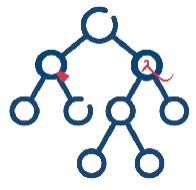
\includegraphics[height=1.0cm]{msca_logo.png}}%
    \end{center}

    \vspace{0.6cm}

    % Main title with Q logos on sides (with clickable links)
    \begin{center}
        \begin{minipage}{0.1\textwidth}
            \centering
            \href{https://quantlet.com}{
\includegraphics[height=1.1cm]{ql_logo.png}}
        \end{minipage}%
        \begin{minipage}{0.78\textwidth}
            \centering
            {\LARGE\bfseries\usebeamercolor[fg]{title}\inserttitle}

            \vspace{0.3cm}

            {\usebeamerfont{subtitle}\usebeamercolor[fg]{title}\insertsubtitle}
        \end{minipage}%
        \begin{minipage}{0.1\textwidth}
            \centering
            \href{https://quantinar.com}{
\includegraphics[height=1.1cm]{qr_logo.png}}
        \end{minipage}
    \end{center}

    \vspace{0.6cm}

    % Authors (left aligned)
    \hspace{0.5cm}{\usebeamerfont{author}\insertauthor}

    \vspace{0.3cm}

    % Institute/Affiliations (left aligned)
    \hspace{0.5cm}\begin{minipage}[t]{0.9\textwidth}
        \raggedright\small\insertinstitute
    \end{minipage}
}

%=============================================================================
% THEOREM ENVIRONMENTS
%=============================================================================
\theoremstyle{definition}
\setbeamertemplate{theorems}[numbered]
\ifdefined\sfmlang
\newtheorem{defn}{Definiție}
\newtheorem{thm}{Teoremă}
\newtheorem{prop}{Propoziție}
\newtheorem{rmk}{Observație}
\else
\newtheorem{defn}{Definition}
\newtheorem{thm}{Theorem}
\newtheorem{prop}{Proposition}
\newtheorem{rmk}{Remark}
\fi

%=============================================================================
% CENTRED MINIPAGE (no extra vertical space)
%=============================================================================
\newenvironment{cminipage}[1]{%
    \par\noindent\hfill\begin{minipage}{#1}\ignorespaces
}{%
    \end{minipage}\hfill\null\par
}

%=============================================================================
% CUSTOM COMMANDS
%=============================================================================
\newcommand{\E}{\mathbb{E}}
\newcommand{\Var}{\text{Var}}
\newcommand{\Cov}{\text{Cov}}
\newcommand{\Corr}{\text{Corr}}
\newcommand{\R}{\mathbb{R}}
\newcommand{\N}{\mathbb{N}}
\newcommand{\Z}{\mathbb{Z}}
\newcommand{\B}{\mathbf{B}}
\newcommand{\imark}{\textcolor{MainBlue}{\textbullet}}
\newcommand{\RMSE}{\text{RMSE}}
\newcommand{\MAE}{\text{MAE}}
\newcommand{\MAPE}{\text{MAPE}}



\newcommand{\qlurl}[1]{https://github.com/danpele/SFM/tree/main/Quantlets/Ch_03/#1}

\DeclareUnicodeCharacter{03B1}{\ensuremath{\alpha}}

% Clickable citations (DOIs verified via Crossref)

\newcommand{\refMandelbrot}{\href{https://doi.org/10.1086/294632}{Mandelbrot (1963)}}
\newcommand{\refFama}{\href{https://doi.org/10.1086/294743}{Fama (1965)}}
\newcommand{\refFamaRoll}{\href{https://doi.org/10.1080/01621459.1968.11009311}{Fama \& Roll (1968)}}
\newcommand{\refFamaRollB}{\href{https://doi.org/10.1080/01621459.1971.10482264}{Fama \& Roll (1971)}}
\newcommand{\refCMS}{\href{https://doi.org/10.1080/01621459.1976.10480344}{Chambers, Mallows \& Stuck (1976)}}
\newcommand{\refWeron}{\href{https://doi.org/10.1016/0167-7152(95)00113-1}{Weron (1996)}}
\newcommand{\refMcCulloch}{\href{https://doi.org/10.1080/03610918608812563}{McCulloch (1986)}}
\newcommand{\refNolanA}{\href{https://doi.org/10.1080/15326349708807450}{Nolan (1997)}}
\newcommand{\refNolan}{\href{https://doi.org/10.1007/978-3-030-52915-4}{Nolan (2020)}}
\newcommand{\refNolanML}{\href{https://doi.org/10.1007/978-1-4612-0197-7_17}{Nolan (2001)}}
\newcommand{\refST}{\href{https://doi.org/10.1201/9780203738818}{Samorodnitsky \& Taqqu (1994)}}
\newcommand{\refBHW}{\href{https://doi.org/10.1007/3-540-27395-6_1}{Borak, Härdle \& Weron (2005)}}
\newcommand{\refBMW}{\href{https://doi.org/10.1007/978-3-642-18062-0_1}{Borak, Misiorek \& Weron (2011)}}
\newcommand{\refFHH}{\href{https://doi.org/10.1007/978-3-030-13751-9}{Franke, Härdle \& Hafner (2019)}}
\newcommand{\refOfficer}{\href{https://doi.org/10.1080/01621459.1972.10481297}{Officer (1972)}}
\newcommand{\refBG}{\href{https://doi.org/10.1086/295634}{Blattberg \& Gonedes (1974)}}
\newcommand{\refAB}{\href{https://doi.org/10.1080/07350015.1988.10509636}{Akgiray \& Booth (1988)}}
\newcommand{\refLLW}{\href{https://doi.org/10.1080/07350015.1990.10509793}{Lau, Lau \& Wingender (1990)}}
\newcommand{\refCont}{\href{https://doi.org/10.1080/713665670}{Cont (2001)}}
\newcommand{\refRM}{\href{https://www.wiley.com/en-us/Stable+Paretian+Models+in+Finance-p-9780471953142}{Rachev \& Mittnik (2000)}}
\newcommand{\refMDC}{\href{https://doi.org/10.1016/S0895-7177(99)00106-5}{Mittnik, Doganoglu \& Chenyao (1999)}}
\newcommand{\refMRDC}{\href{https://doi.org/10.1016/S0895-7177(99)00110-7}{Mittnik et al.\ (1999)}}
\newcommand{\refKoutrouvelis}{\href{https://doi.org/10.1080/01621459.1980.10477573}{Koutrouvelis (1980)}}
\newcommand{\refMS}{\href{https://doi.org/10.1038/376046a0}{Mantegna \& Stanley (1995)}}
\newcommand{\refGopi}{\href{https://doi.org/10.1103/PhysRevE.60.5305}{Gopikrishnan et al.\ (1999)}}
\newcommand{\refWang}{\href{https://doi.org/10.1038/s41586-023-06221-2}{Wang et al.\ (2023)}}
\newcommand{\refGS}{\href{https://doi.org/10.1080/14697680903540381}{Grabchak \& Samorodnitsky (2010)}}
\newcommand{\refHill}{\href{https://doi.org/10.1214/aos/1176343247}{Hill (1975)}}
\newcommand{\refGK}{\href{https://archive.org/details/limitdistributio00gned_0}{Gnedenko \& Kolmogorov (1954)}}
\newcommand{\refPele}{\href{https://doi.org/10.1016/S2212-5671(14)00279-2}{Pele (2014)}}

\title[Statistics of Financial Markets]{Statistics of Financial Markets}
\subtitle{Chapter 3: α-stable distributions}
\author[D.T. Pele]{Daniel Traian PELE}
\institute{Bucharest University of Economic Studies\\
IDA Institute Digital Assets\\
Blockchain Research Center\\
AI4EFin Artificial Intelligence for Energy Finance\\
Romanian Academy, Institute for Economic Forecasting\\
MSCA Digital Finance}
\date{}

%=============================================================================
\providecommand{\sfmapplink}[3]{\hypertarget{#2}{}\hyperlink{#1}{\beamergotobutton{#3}}}  % APPLINKS-MACROS
\providecommand{\sfmappback}[2]{\begin{tikzpicture}[remember picture,overlay]\node[anchor=south east] at ([xshift=-3mm,yshift=7mm]current page.south east){\hyperlink{#1}{\beamerreturnbutton{#2}}};\end{tikzpicture}}  % APPLINKS-MACROS
\providecommand{\sfmchlink}[2]{\href{#1}{#2}}  % APPLINKS-MACROS
\providecommand{\sfmchlinkt}[2]{\href{#1}{\usebeamercolor[fg]{frametitle}#2}}  % APPLINKS-MACROS
\begin{document}
%=============================================================================

{
\setbeamertemplate{headline}{}
\setbeamertemplate{footline}{}
\begin{frame}[noframenumbering]
    \titlepage
\end{frame}
}
% BEGIN-ACRONYMS (generat de latex/acronyms.py; nu editati manual)
\begin{frame}{Acronyms used in this material}
\setbeamertemplate{itemize/enumerate body begin}{\tiny}
\begin{columns}[T]
\begin{column}{0.49\textwidth}
\begin{itemize}\setlength{\itemsep}{0pt}
    \item \textbf{AI}: Artificial Intelligence
    \item \textbf{AIC}: Akaike Information Criterion
    \item \textbf{BET}: Bucharest Exchange Trading (index)
    \item \textbf{CLT}: Central Limit Theorem
    \item \textbf{CMS}: Chambers–Mallows–Stuck (simulation method)
    \item \textbf{EODHD}: EOD Historical Data (market-data provider)
    \item \textbf{ES}: Expected Shortfall
    \item \textbf{FFT}: Fast Fourier Transform
    \item \textbf{GCLT}: Generalised Central Limit Theorem
    \item \textbf{IBM}: International Business Machines (company)
    \item \textbf{KS}: Kolmogorov–Smirnov (test)
    \item \textbf{ML}: Maximum Likelihood
    \item \textbf{QQ}: Quantile–Quantile (plot)
\end{itemize}
\end{column}
\begin{column}{0.49\textwidth}
\begin{itemize}\setlength{\itemsep}{0pt}
    \item \textbf{SAS}: Statistical Analysis System (software)
    \item \textbf{SE}: Standard Error
\end{itemize}
\end{column}
\end{columns}
\end{frame}
% END-ACRONYMS

\begin{frame}{Today's Question and Route}
\itemsize{\small}
\begin{itemize}
    \item \textbf{Question}: which probability laws can describe daily returns and also their weekly and monthly sums?
    \begin{itemize}
        \item \sfmchlink{https://danpele.github.io/SFM/EN/Courses/chapter2_classical_distributions_stylised_facts.pdf}{Chapter 2}: daily returns have heavier tails than the Normal distribution
        \item log returns add up over time (\sfmchlink{https://danpele.github.io/SFM/EN/Courses/chapter1_data_returns_indicators.pdf}{Chapter 1}): the law of a sum matters
    \end{itemize}
    \item \textbf{Route} of the chapter
    \begin{itemize}
        \item Mandelbrot and the cotton prices: where the idea comes from
        \item stability under summation and the generalised central limit theorem
        \item parameters, characteristic function, tails and moments
        \item simulation and estimation; fits to BET, S\&P 500, DAX and Bitcoin
        \item the critique: do returns really have infinite variance?
    \end{itemize}
\end{itemize}
\end{frame}

\begin{frame}{Learning Outcomes}
\itemsize{\small}
\begin{itemize}
    \item State the stability property and compute the scale of a sum of stable variables
    \item Explain the generalised central limit theorem and when sums do not approach the Normal distribution
    \item Read the four parameters $(\alpha, \beta, \gamma, \delta)$ and convert between the S0 and S1 parameterisations
    \item Say which moments exist for a given $\alpha$ and compare tail probabilities with the Normal distribution
    \item Simulate stable variables and estimate their parameters by quantiles and by maximum likelihood
    \item Judge, on real returns, where the stable model works and where it fails
\end{itemize}
\end{frame}

\begin{frame}{Reading and Tools}
\itemsize{\small}
\begin{itemize}
    \item Main reference: \refNolan, Ch.~1 (definitions, parameterisations, tails) and Ch.~4 (estimation)
    \begin{itemize}
        \item short survey with code: \refBHW; updated in \refBMW
    \end{itemize}
    \item Textbook: \refFHH, Ch.~3 (probability) and Ch.~18 (heavy tails and extreme risks)
    \item The original papers: \refMandelbrot, \refFama
    \item Python Quantlets of this chapter: \href{https://github.com/danpele/SFM/tree/main/Quantlets/Ch_03}{Quantlets/Ch\_03}
    \begin{itemize}
        \item ported from the Quantlet sim\_stable; each chart links to the Quantlet that draws it
    \end{itemize}
    \item Lecture notebook: \href{\colaburl{notebooks/EN/chapter3_lecture_notebook.ipynb}}{open in Google Colab}
    \item Video course: \quantinar{Stable Distribution}{https://quantinar.com/course/980/stable-distribution}
\end{itemize}
\end{frame}


%=============================================================================
\section{Mandelbrot and the Cotton Prices}
%=============================================================================

\begin{frame}{Cotton: an Old Market with Long Price Records}
\itemsize{\small}
\begin{columns}[T]
\begin{column}{0.52\textwidth}
\begin{itemize}
    \item In the 19th century cotton was one of the most traded commodities in the world
    \begin{itemize}
        \item exchanges in New Orleans, New York and Liverpool quoted prices every day
        \item the result: some of the longest daily and monthly price series in economics
    \end{itemize}
    \item In the early 1960s these series reached Benoit Mandelbrot, then at IBM
    \begin{itemize}
        \item he looked at the \textbf{changes} of the logarithm of the price, i.e.\ log returns
    \end{itemize}
    \item His paper \refMandelbrot\ started the study of heavy tails in finance
\end{itemize}
\end{column}
\begin{column}{0.44\textwidth}
\centering
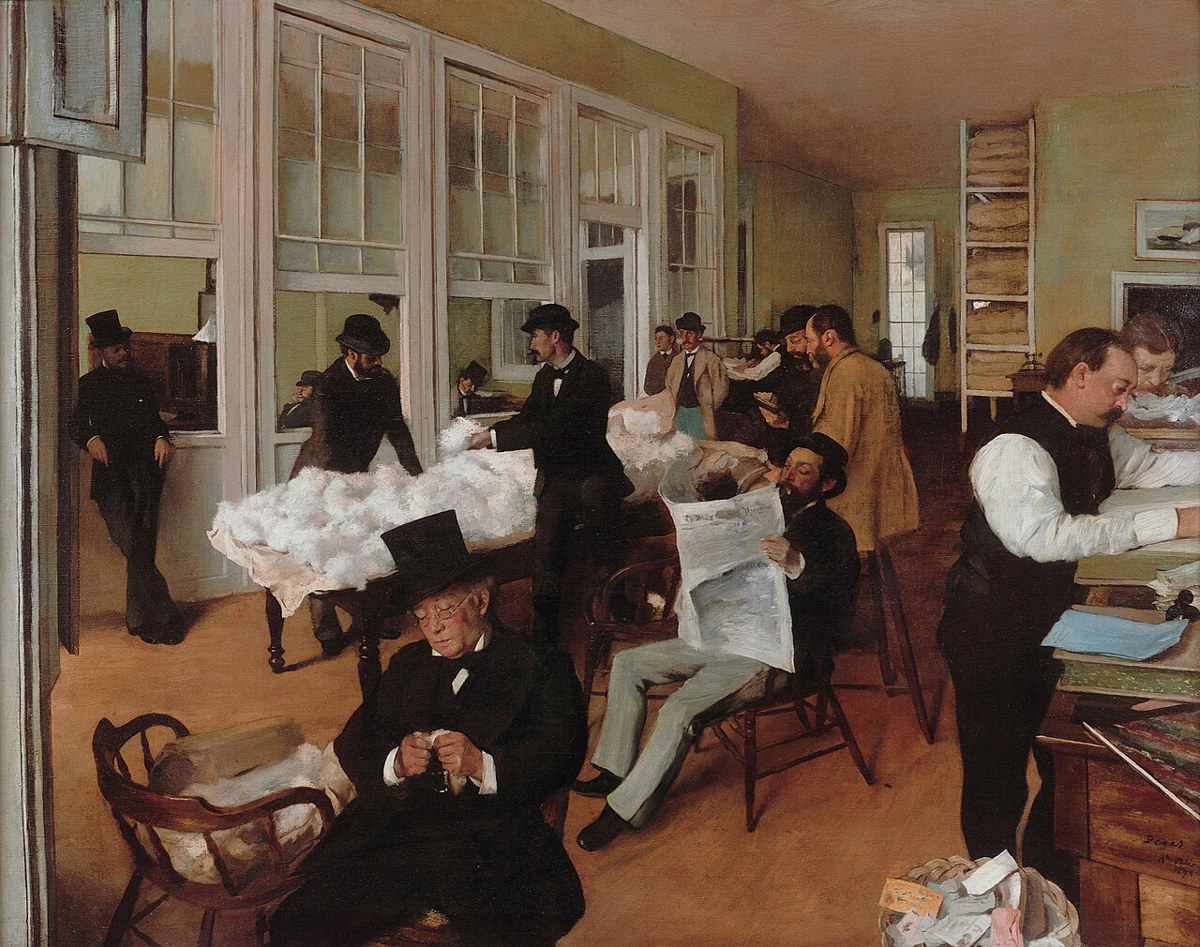
\includegraphics[height=0.42\textheight]{ch3_cotton_office.jpg}\\[1mm]
\imgcap{Edgar Degas, A Cotton Office in New Orleans (1873)}
\imgcredit{https://commons.wikimedia.org/wiki/File:Edgar_Germain_Hilaire_Degas_016.jpg}{Image: Edgar Degas (1873); public domain; Wikimedia Commons}
\end{column}
\end{columns}
\end{frame}

\begin{frame}{What Mandelbrot Saw}
\itemsize{\small}
\begin{columns}[T]
\begin{column}{0.62\textwidth}
\begin{itemize}
    \item \textbf{Too many large changes}: far more big moves than the Normal distribution allows
    \begin{itemize}
        \item the sample variance did not settle as the sample grew
    \end{itemize}
    \item \textbf{The same shape at every horizon}: daily and monthly changes looked alike after rescaling
    \begin{itemize}
        \item a sum of many daily changes kept the shape of one daily change
    \end{itemize}
    \item \textbf{His proposal}: stable Paretian laws with $\alpha \approx 1.7$ \refMandelbrot
    \begin{itemize}
        \item ``Paretian'': the tails decay like a power of $x$, as in Pareto's law of incomes
        \item consequence: the variance of price changes would be infinite
    \end{itemize}
\end{itemize}
\end{column}
\begin{column}{0.34\textwidth}
\centering

\includegraphics[height=0.45\textheight]{ch3_mandelbrot.jpg}\\[1mm]
\imgcap{Benoit Mandelbrot (1924--2010)}
\imgcredit{https://commons.wikimedia.org/wiki/File:Benoit_Mandelbrot_mg_1804-d.jpg}{Photo: Rama (2007); CC BY-SA 2.0 fr; Wikimedia Commons}
\end{column}
\end{columns}
\end{frame}

\begin{frame}{Fama Tests the Idea on Stocks}
\itemsize{\small}
\begin{columns}[T]
\begin{column}{0.62\textwidth}
\begin{itemize}
    \item \refFama: daily returns of the 30 stocks of the Dow Jones Industrial Average
    \begin{itemize}
        \item more large returns than the Normal distribution predicts, for every stock
        \item estimates of $\alpha$ below 2: support for Mandelbrot's hypothesis
    \end{itemize}
    \item Estimation methods for symmetric stable laws followed
    \begin{itemize}
        \item \refFamaRoll, \refFamaRollB: quantile-based estimates and tables
    \end{itemize}
    \item Within ten years the evidence started to turn: see the critique at the end of the chapter
\end{itemize}
\end{column}
\begin{column}{0.34\textwidth}
\centering

\includegraphics[height=0.45\textheight]{ch3_fama.jpg}\\[1mm]
\imgcap{Eugene Fama at the Nobel Prize ceremony, 2013}
\imgcredit{https://commons.wikimedia.org/wiki/File:Eugene_Fama_at_Nobel_Prize,_2013.jpg}{Photo: Bengt Nyman (2013); CC BY 2.0; Wikimedia Commons}
\end{column}
\end{columns}
\end{frame}

\begin{frame}{Why the Law of a Sum Matters}
\itemsize{\small}
\begin{itemize}
    \item A monthly log return is the sum of about 21 daily log returns
    \begin{itemize}
        \item a model for daily returns implies a model for weekly, monthly and yearly returns
    \end{itemize}
    \item The Normal distribution keeps its shape under summation (\sfmchlink{https://danpele.github.io/SFM/EN/Courses/chapter2_classical_distributions_stylised_facts.pdf}{Chapter 2})
    \begin{itemize}
        \item but it has thin tails: it misses the large daily moves
    \end{itemize}
    \item \textbf{Question for the room}: the Student-t distribution has heavy tails; is a sum of 21 independent Student-t variables again Student-t?
    \item \textbf{Answer}
    \begin{itemize}
        \item no: the Student-t family is not closed under summation
        \item if its variance is finite, the sum moves towards the Normal distribution (the central limit theorem)
    \end{itemize}
    \item \textbf{Goal}: find every law whose sums keep the same shape
\end{itemize}
\end{frame}


%=============================================================================
\section{Stability under Summation}
%=============================================================================

\begin{frame}{Definition: Stable Laws}
\itemsize{\small}
\begin{itemize}
    \item $X$ is \textbf{stable} if, for $X_1, X_2$ independent copies of $X$ and any $a, b > 0$, there are $c > 0$ and $d$ with
    \begin{itemize}
        \item $aX_1 + bX_2 \overset{d}{=} cX + d$, where $\overset{d}{=}$ means ``has the same distribution as''
        \item $a, b$: the weights of the two copies; $c$: the scale and $d$: the shift of the result
        \item \textbf{strictly stable} if $d = 0$ for all $a, b$
    \end{itemize}
    \item In words: a weighted sum of two copies has the same shape as one copy
    \begin{itemize}
        \item only the scale ($c$) and the location ($d$) change
    \end{itemize}
    \item By induction, for $n$ independent copies: $X_1 + \dots + X_n \overset{d}{=} c_n X + d_n$
    \begin{itemize}
        \item the only possible scale factor is $c_n = n^{1/\alpha}$ with $0 < \alpha \le 2$ \refNolan
    \end{itemize}
    \item $\alpha$ is called the \textbf{index of stability} (also: characteristic exponent, tail index)
\end{itemize}
\end{frame}

\begin{frame}{Two Examples: Normal and Cauchy}
\itemsize{\small}
\begin{columns}[T]
\begin{column}{0.64\textwidth}
\begin{itemize}
    \item \textbf{Normal}: $X_1, X_2 \sim N(0, \sigma^2)$ independent
    \begin{itemize}
        \item $aX_1 + bX_2 \sim N(0, (a^2 + b^2)\sigma^2)$, so $c = \sqrt{a^2 + b^2}$
        \item variances add: $c^2 = a^2 + b^2$, the case $\alpha = 2$
    \end{itemize}
    \item \textbf{Cauchy}: density $f(x) = \dfrac{1}{\pi(1 + x^2)}$
    \begin{itemize}
        \item $aX_1 + bX_2$ is Cauchy with scale $c = a + b$
        \item scales add linearly: $c^1 = a^1 + b^1$, the case $\alpha = 1$
        \item the average of $n$ Cauchy draws is again standard Cauchy: averaging does not help
    \end{itemize}
\end{itemize}
\end{column}
\begin{column}{0.32\textwidth}
\centering
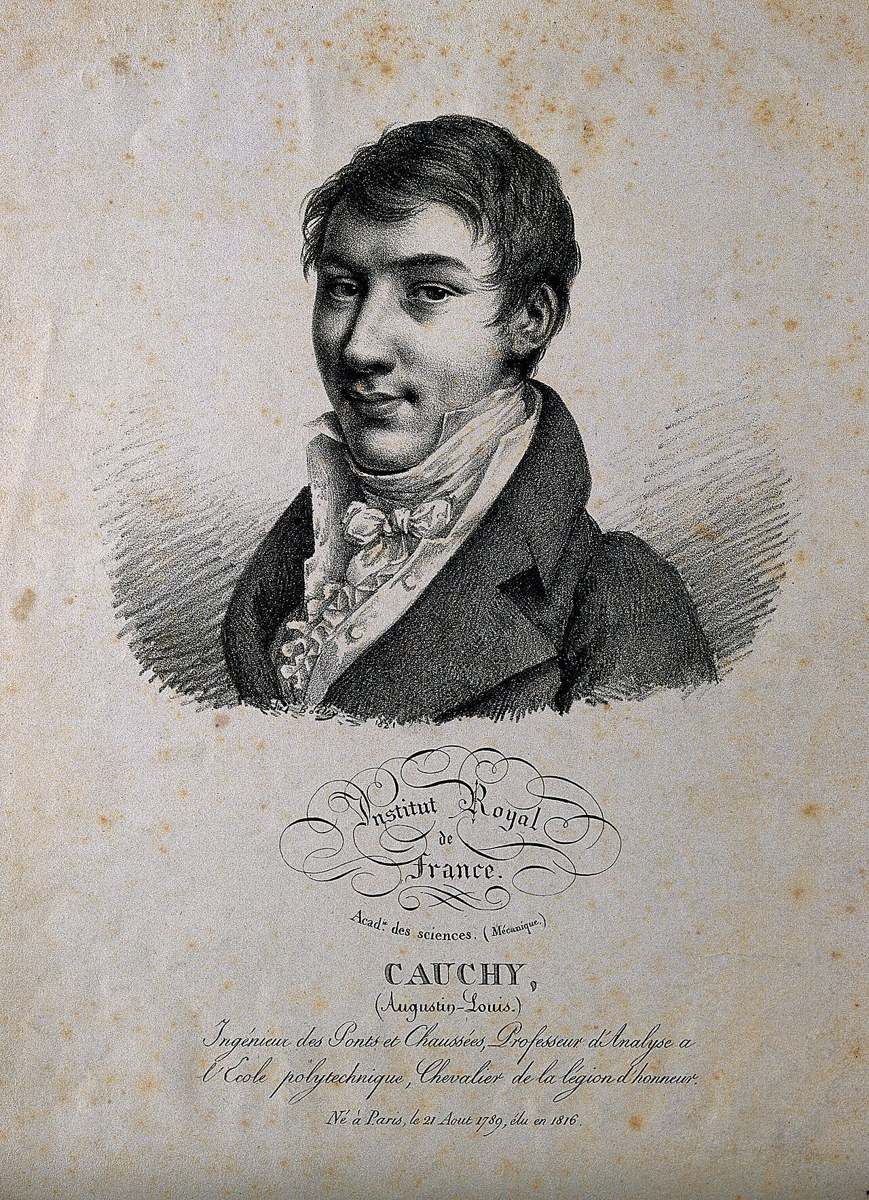
\includegraphics[height=0.46\textheight]{ch3_cauchy.jpg}\\[1mm]
\imgcap{Augustin-Louis Cauchy (1789--1857)}
\imgcredit{https://commons.wikimedia.org/wiki/File:Augstin_Louis,_Baron_Cauchy._Lithograph_by_J._Boilly,_1821._Wellcome_V0001034.jpg}{Lithograph: J. Boilly (1821), Wellcome Collection; CC BY 2.0; Wikimedia Commons}
\end{column}
\end{columns}
\end{frame}

\begin{frame}{The General Rule and a Worked Example}
\itemsize{\small}
\begin{itemize}
    \item For $X_1, X_2$ independent copies of a strictly stable $X$ with index $\alpha$:
    \begin{itemize}
        \item $c^\alpha = a^\alpha + b^\alpha$, i.e.\ $c = (a^\alpha + b^\alpha)^{1/\alpha}$
    \end{itemize}
    \item \textbf{Example}: $a = 3$, $b = 4$
    \begin{itemize}
        \item $\alpha = 2$: $c = \sqrt{9 + 16} = 5.00$
        \item $\alpha = 1.5$: $c = (3^{1.5} + 4^{1.5})^{1/1.5} = 5.58$
        \item $\alpha = 1$: $c = 3 + 4 = 7.00$
    \end{itemize}
    \item The smaller $\alpha$, the larger the scale of the sum: one large term can dominate the sum
    \item \textbf{What do you think?} For $\alpha = 1.5$, what is the scale factor of a sum of two copies?
    \item \textbf{Answer}
    \begin{itemize}
        \item $c_2 = 2^{1/1.5} = 2^{2/3} = 1.59$, larger than $\sqrt{2} \approx 1.41$ for the Normal distribution
    \end{itemize}
\end{itemize}
\end{frame}

\begin{frame}{Stability in a Simulation}
\itemsize{\footnotesize}
\begin{center}
    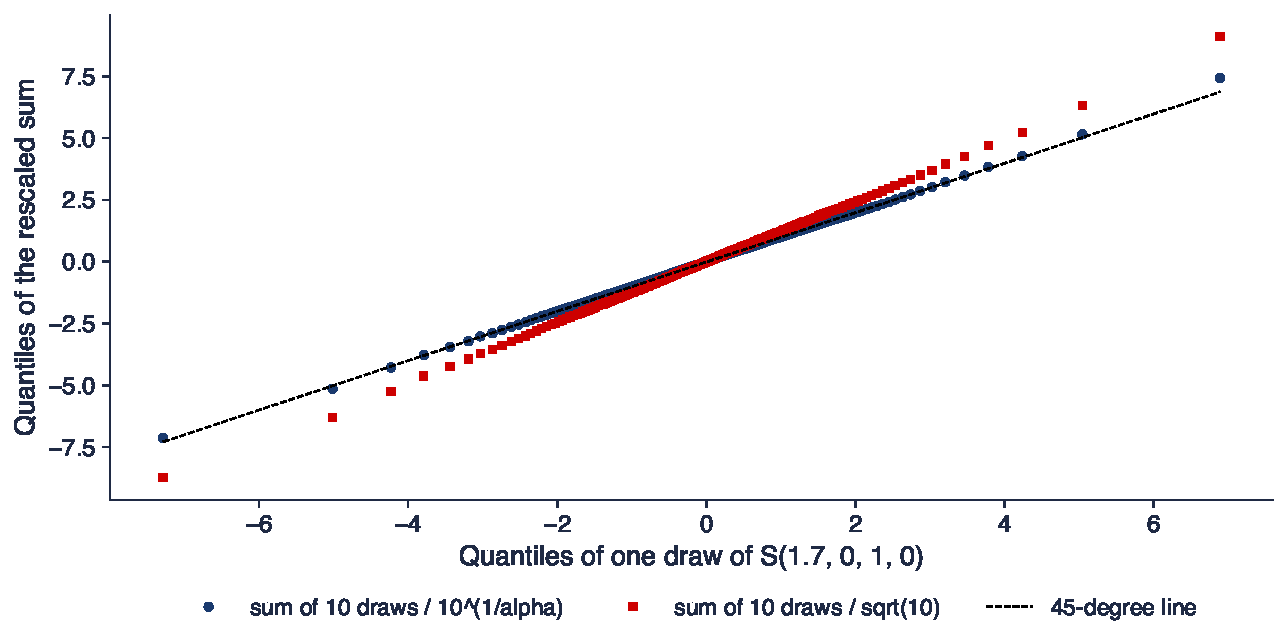
\includegraphics[width=0.97\textwidth,height=0.64\textheight,keepaspectratio]{sfm_ch3_stability_qq.pdf}
\end{center}
\vspace{-0.25cm}
\begin{itemize}
    \item Notation (Section 4): $S(\alpha, \beta, \gamma, \delta)$ is the stable law with index $\alpha$, skewness $\beta$, scale $\gamma$ and location $\delta$
    \item Blue: sums of 10 draws of $S(1.7, 0, 1, 0)$ divided by $10^{1/1.7} = 3.87$ lie on the 45-degree line: same law as one draw
    \item Red: dividing by $\sqrt{10} = 3.16$ (the Normal rule) leaves the tails too wide: 99\% quantile $6.31$ vs $5.04$
\end{itemize}
\quantlet{SFM\_ch3\_stability\_gclt}{\qlurl{SFM_ch3_stability_gclt}}
\end{frame}

\begin{frame}{Consequences: Horizons and Diversification}
\itemsize{\small}
\begin{itemize}
    \item \textbf{Horizon}: if daily returns are i.i.d.\ (independent, identically distributed) $S(\alpha, 0, \gamma, 0)$, the 20-day sum has scale $20^{1/\alpha}\gamma$
    \begin{itemize}
        \item $\alpha = 2$: $4.47\,\gamma$ (the square-root-of-time rule); $\alpha = 1.7$: $5.83\,\gamma$; $\alpha = 1.5$: $7.37\,\gamma$
        \item with $\alpha < 2$, the risk of long horizons grows faster than $\sqrt{n}$
    \end{itemize}
    \item \textbf{Diversification}: an equally weighted portfolio of $N$ i.i.d.\ stable assets has scale $N^{1/\alpha - 1}\gamma$
    \begin{itemize}
        \item $N = 10$: $\alpha = 2$ gives $0.32\,\gamma$; $\alpha = 1.5$ gives $0.46\,\gamma$; $\alpha = 1$ gives $1.00\,\gamma$
        \item with $\alpha = 1$ diversification does not reduce the scale at all; \refFama\ discussed this point
    \end{itemize}
\end{itemize}
\end{frame}

\begin{frame}{Recap: Stability}
\itemsize{\small}
\begin{itemize}
    \item Stable law: a sum of independent copies has the same shape, only rescaled and shifted
    \item Scale rule: $c^\alpha = a^\alpha + b^\alpha$; $n$ copies: factor $n^{1/\alpha}$, $0 < \alpha \le 2$
    \item Normal: $\alpha = 2$; Cauchy: $\alpha = 1$
    \item Small $\alpha$: risk grows faster with the horizon and diversification helps less
\end{itemize}
\end{frame}


%=============================================================================
\section{The Generalised Central Limit Theorem}
%=============================================================================

\begin{frame}{From the Classical to the Generalised CLT}
\itemsize{\small}
\begin{itemize}
    \item \textbf{Classical CLT} (central limit theorem, \sfmchlink{https://danpele.github.io/SFM/EN/Courses/chapter2_classical_distributions_stylised_facts.pdf}{Chapter 2}): $X_i$ i.i.d.\ with mean $\mu$ and finite variance $\sigma^2$
    \begin{itemize}
        \item $\dfrac{X_1 + \dots + X_n - n\mu}{\sigma\sqrt{n}} \to N(0, 1)$ in distribution
    \end{itemize}
    \item What if the variance is infinite? The normalisation $\sqrt{n}$ is then wrong
    \item \textbf{GCLT} (generalised central limit theorem) \refGK: if $(X_1 + \dots + X_n - b_n)/a_n$ converges to a non-degenerate law, that law is stable
    \begin{itemize}
        \item $a_n > 0$, $b_n$: normalising constants that rescale and recentre the sum (for the classical CLT, $a_n = \sigma\sqrt{n}$, $b_n = n\mu$)
        \item stable laws are the \textbf{only} possible limits of normalised sums of i.i.d.\ variables
        \item the Normal distribution is the special case $\alpha = 2$
    \end{itemize}
\end{itemize}
\end{frame}

\begin{frame}{Domains of Attraction}
\itemsize{\small}
\begin{columns}[T]
\begin{column}{0.64\textwidth}
\begin{itemize}
    \item The \textbf{domain of attraction} of a stable law: all laws whose normalised sums converge to it
    \begin{itemize}
        \item finite variance: domain of attraction of the Normal distribution, $a_n \propto \sqrt{n}$
        \item power-law tails $P(|X| > x) \approx C x^{-\alpha}$ with $0 < \alpha < 2$: the stable law with the same $\alpha$, $a_n \propto n^{1/\alpha}$
        \item $C > 0$: a constant; $\propto$: proportional to
    \end{itemize}
    \item So the \textbf{tail} of one return decides the law of long sums
    \item Paul Lévy characterised the stable laws in the 1920s; the full theory is in \refGK
\end{itemize}
\end{column}
\begin{column}{0.32\textwidth}
\centering
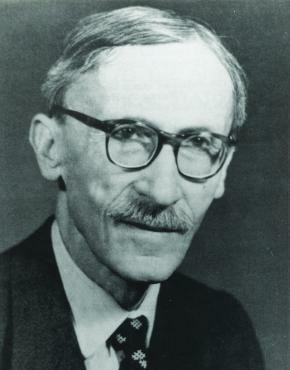
\includegraphics[height=0.42\textheight]{ch3_levy.jpg}\\[1mm]
\imgcap{Paul Lévy (1886--1971)}
\imgcredit{https://commons.wikimedia.org/wiki/File:Paul_Pierre_Levy_1886-1971.jpg}{Photo: Konrad Jacobs, Oberwolfach Photo Collection; CC BY-SA 2.0 de; Wikimedia Commons}
\end{column}
\end{columns}
\end{frame}

\begin{frame}{The GCLT in a Simulation}
\itemsize{\footnotesize}
\begin{center}
    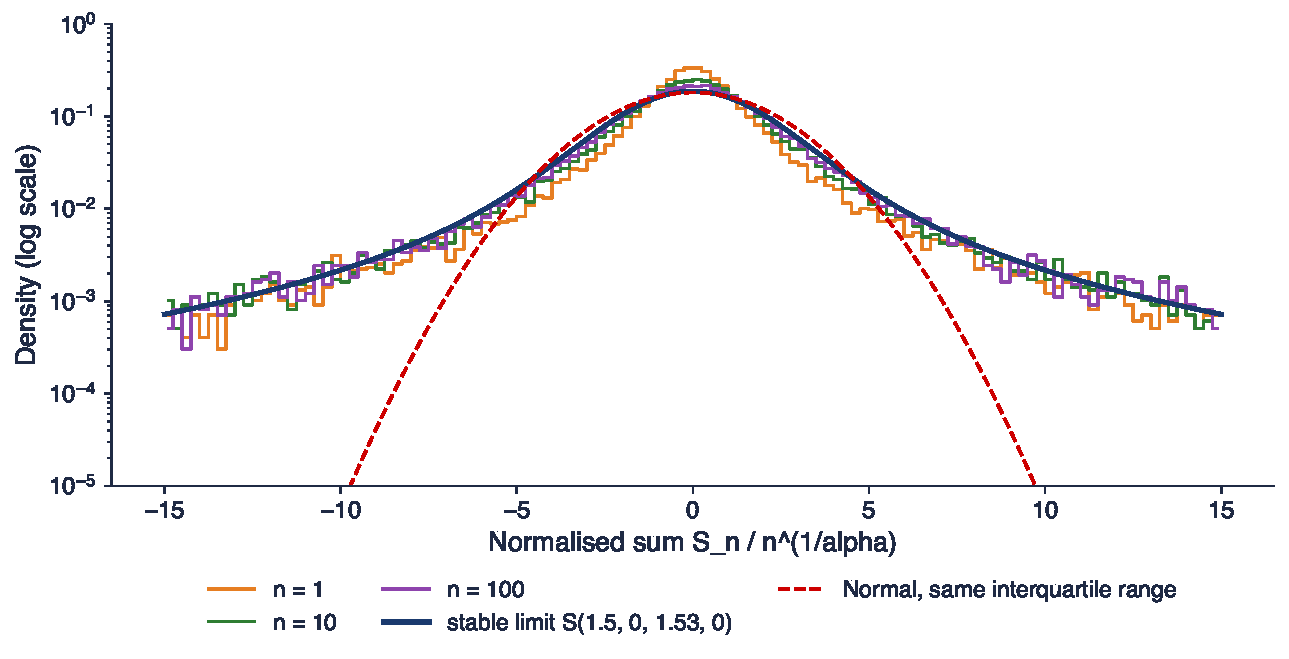
\includegraphics[width=0.97\textwidth,height=0.64\textheight,keepaspectratio]{sfm_ch3_gclt.pdf}
\end{center}
\vspace{-0.25cm}
\begin{itemize}
    \item Student-t with $\nu = 1.5$ degrees of freedom: infinite variance, tails $\propto x^{-1.5}$; sums of $n$ draws divided by $n^{1/1.5}$
    \item $n = 1, 10, 100$: the histograms approach the stable limit $S(1.5, 0, 1.53, 0)$; $P(|\cdot| > 10)$: $2.73\%$ for $n = 100$, $2.64\%$ in the limit
    \item A Normal law with the same interquartile range gives $0.0005\%$: it misses the tails completely
\end{itemize}
\quantlet{SFM\_ch3\_stability\_gclt}{\qlurl{SFM_ch3_stability_gclt}}
\end{frame}

\begin{frame}{What the GCLT Means for Returns}
\itemsize{\small}
\begin{itemize}
    \item Two possible worlds for daily returns
    \begin{itemize}
        \item \textbf{tail index below 2} (infinite variance): monthly returns are stable with the \textbf{same} $\alpha$
        \item \textbf{tail index above 2} (finite variance): monthly returns move towards the Normal distribution
    \end{itemize}
    \item The two worlds give different testable predictions about returns at longer horizons
    \item \textbf{Question for the room}: in which world do the S\&P 500 returns live?
    \item \textbf{Answer}
    \begin{itemize}
        \item we test it with real data in the last sections: estimates of $\alpha$ at daily, weekly and monthly horizons
    \end{itemize}
\end{itemize}
\end{frame}

\begin{frame}{Recap: The Generalised CLT}
\itemsize{\small}
\begin{itemize}
    \item Classical CLT: finite variance, normalisation $\sqrt{n}$, Normal limit
    \item GCLT: stable laws are the only limits of normalised sums
    \item Power-law tails with index $\alpha < 2$: normalisation $n^{1/\alpha}$, stable limit with the same $\alpha$
    \item The tail of a single return decides the law of long sums
\end{itemize}
\end{frame}


%=============================================================================
\section{Parameters and the Characteristic Function}
%=============================================================================

\begin{frame}{The Characteristic Function}
\itemsize{\small}
\begin{itemize}
    \item \textbf{Characteristic function} of $X$: $\varphi_X(t) = E[e^{itX}] = E[\cos(tX)] + i\,E[\sin(tX)]$, $t \in \mathbb{R}$
    \begin{itemize}
        \item $i = \sqrt{-1}$: the imaginary unit; $t$: a real argument, not time
        \item it always exists, because $|e^{itX}| = 1$, even when no moment exists
        \item it determines the distribution uniquely
    \end{itemize}
    \item Two properties used in this chapter
    \begin{itemize}
        \item independent $X, Y$: $\varphi_{X+Y}(t) = \varphi_X(t)\,\varphi_Y(t)$: sums become products
        \item $\varphi_{aX+b}(t) = e^{ibt}\varphi_X(at)$
    \end{itemize}
    \item Normal $N(\mu, \sigma^2)$: $\varphi(t) = \exp(i\mu t - \sigma^2 t^2/2)$
    \item Why we need it: apart from three cases, stable laws have \textbf{no closed-form density}; they are defined by $\varphi$
\end{itemize}
\end{frame}

\begin{frame}{The Stable Characteristic Function (S1)}
\itemsize{\small}
\begin{itemize}
    \item $X \sim S(\alpha, \beta, \gamma, \delta; 1)$ if, for $\alpha \ne 1$, \refST, \refNolan:
    \begin{itemize}
        \item $\varphi(t) = \exp\Big\{-\gamma^\alpha |t|^\alpha \big[1 - i\beta\,\mathrm{sign}(t)\tan\frac{\pi\alpha}{2}\big] + i\delta t\Big\}$
        \item for $\alpha = 1$: $\varphi(t) = \exp\Big\{-\gamma |t| \big[1 + i\beta\,\frac{2}{\pi}\mathrm{sign}(t)\ln|t|\big] + i\delta t\Big\}$
    \end{itemize}
    \item The four parameters
    \begin{itemize}
        \item $\alpha \in (0, 2]$: \textbf{index of stability}; smaller $\alpha$, heavier tails
        \item $\beta \in [-1, 1]$: \textbf{skewness}; $\beta > 0$ heavier right tail, $\beta < 0$ heavier left tail
        \item $\gamma > 0$: \textbf{scale} (it plays the role of $\sigma$); $\delta \in \mathbb{R}$: \textbf{location}
    \end{itemize}
    \item $\mathrm{sign}(t)$: $+1$ for $t > 0$, $-1$ for $t < 0$; the term with $\beta$ makes the law asymmetric
    \item Stability is visible: $\varphi(t)^n$ has the same form, with $\gamma^\alpha$ replaced by $n\gamma^\alpha$
\end{itemize}
\end{frame}

\begin{frame}{The Effect of $\alpha$}
\itemsize{\footnotesize}
\begin{center}
    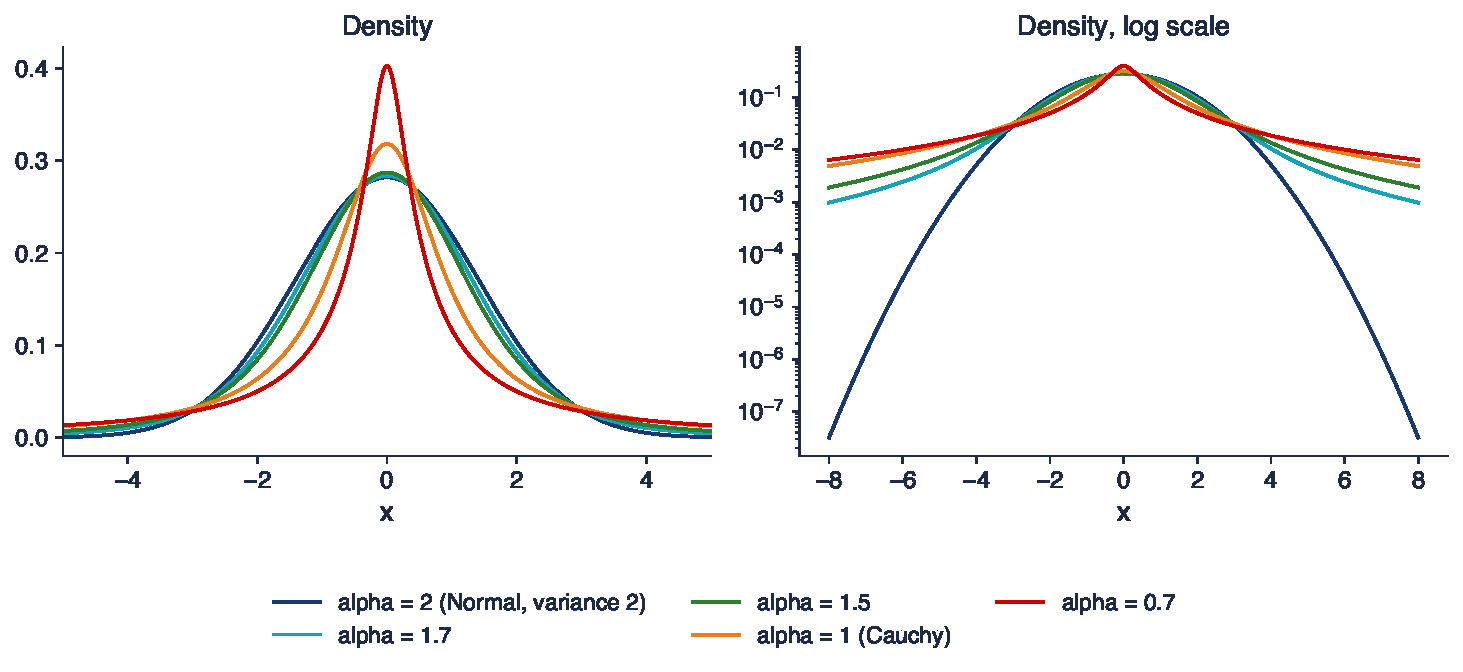
\includegraphics[width=0.97\textwidth,height=0.64\textheight,keepaspectratio]{sfm_ch3_density_alpha.pdf}
\end{center}
\vspace{-0.25cm}
\begin{itemize}
    \item Symmetric laws $S(\alpha, 0, 1, 0)$: smaller $\alpha$ gives a taller, narrower peak and much heavier tails
    \item Log scale: the Normal tail ($\alpha = 2$) falls like $e^{-x^2/4}$; the others fall like a power of $x$
\end{itemize}
\quantlet{SFM\_ch3\_densities}{\qlurl{SFM_ch3_densities}}
\end{frame}

\begin{frame}{The Effect of $\beta$ and $\gamma$}
\itemsize{\footnotesize}
\begin{center}
    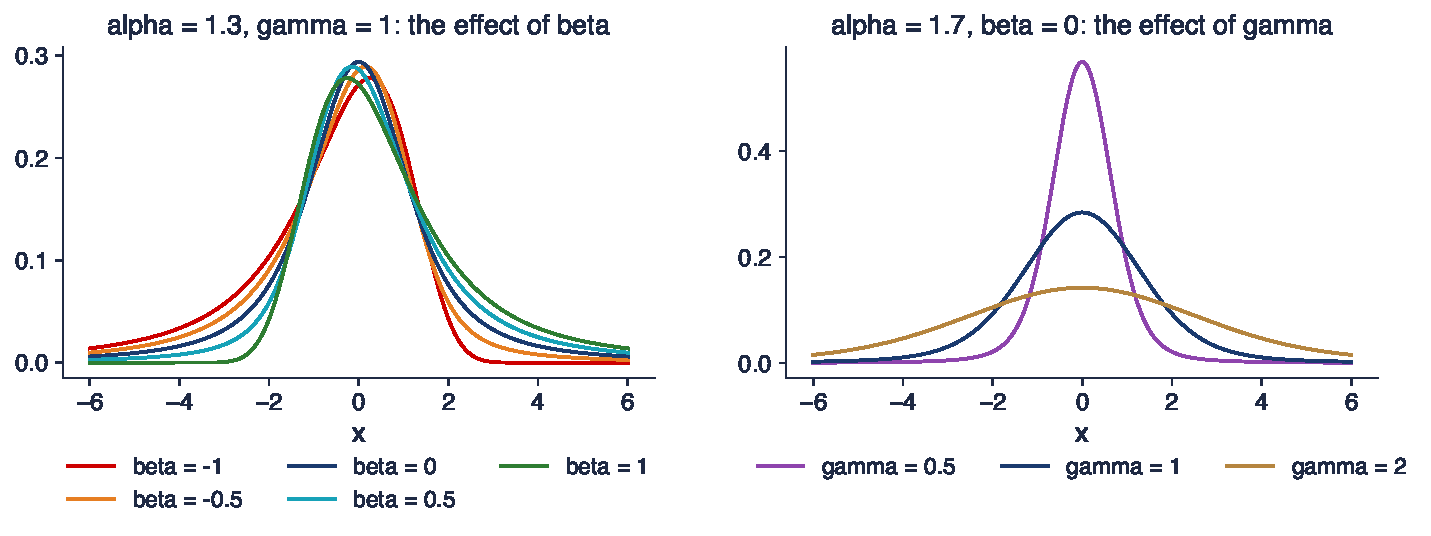
\includegraphics[width=0.97\textwidth,height=0.64\textheight,keepaspectratio]{sfm_ch3_density_beta.pdf}
\end{center}
\vspace{-0.25cm}
\begin{itemize}
    \item $\beta$ moves weight between the tails: $\beta = 1$ (green) has the heavier right tail, $\beta = -1$ (red) the heavier left tail
    \item $\gamma$ stretches the density: doubling $\gamma$ doubles every quantile around $\delta$
\end{itemize}
\quantlet{SFM\_ch3\_densities}{\qlurl{SFM_ch3_densities}}
\end{frame}

\begin{frame}{Two Parameterisations: S0 and S1}
\itemsize{\small}
\begin{itemize}
    \item \textbf{S0} (Nolan's recommendation for data analysis), $\alpha \ne 1$:
    \begin{itemize}
        \item $\varphi(t) = \exp\Big\{-\gamma^\alpha |t|^\alpha \big[1 + i\beta\,\mathrm{sign}(t)\tan\frac{\pi\alpha}{2}\big(|\gamma t|^{1-\alpha} - 1\big)\big] + i\delta_0 t\Big\}$
    \end{itemize}
    \item Only the location differs: $\delta_0 = \delta_1 + \beta\gamma\tan\frac{\pi\alpha}{2}$ ($\alpha \ne 1$)
    \begin{itemize}
        \item $\delta_0$, $\delta_1$: the location parameter in S0 and in S1; $\alpha$, $\beta$ and $\gamma$ are the same in both
        \item for $\beta = 0$ the two coincide
    \end{itemize}
    \item Why two?
    \begin{itemize}
        \item S1: simpler algebra for sums; used in most theory books \refST
        \item S0: the density changes continuously with $\alpha$ and $\beta$; better for estimation and plots \refNolan
    \end{itemize}
\end{itemize}
\end{frame}

\begin{frame}{S1 vs S0 near $\alpha = 1$}
\itemsize{\footnotesize}
\begin{center}
    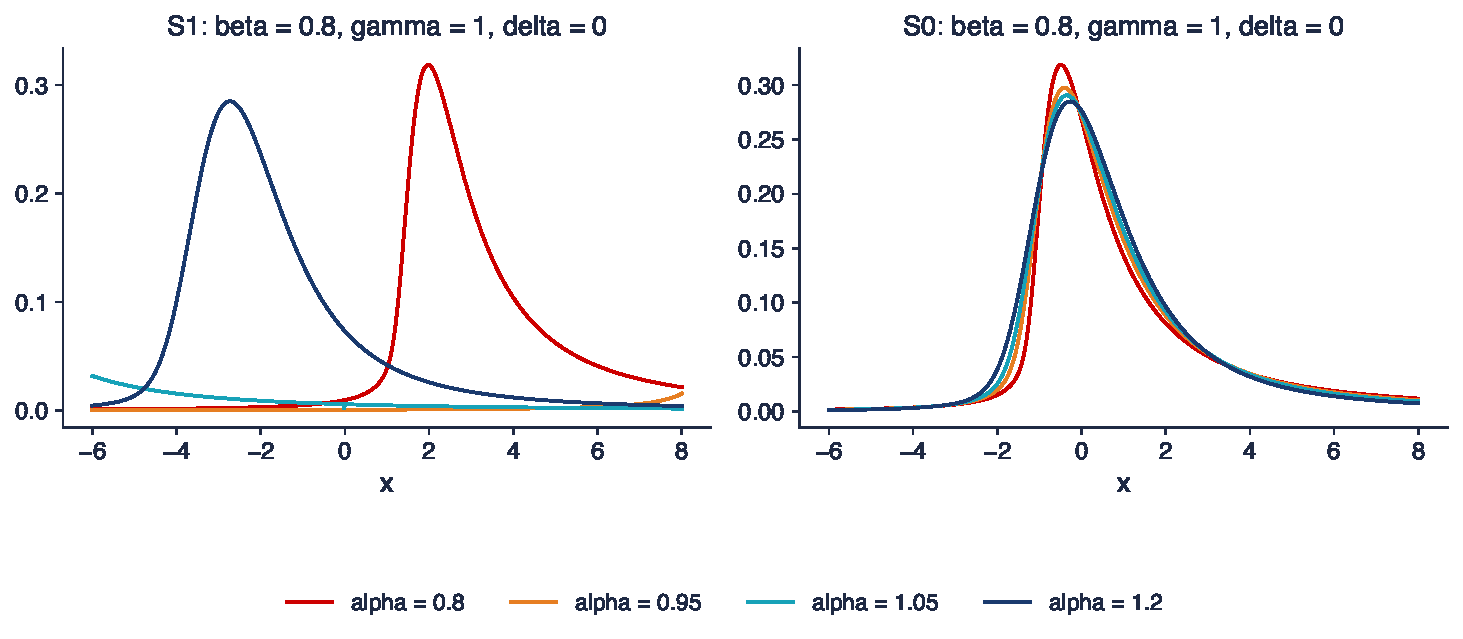
\includegraphics[width=0.97\textwidth,height=0.64\textheight,keepaspectratio]{sfm_ch3_s0_s1.pdf}
\end{center}
\vspace{-0.25cm}
\begin{itemize}
    \item S1 (left): with $\beta = 0.8$, the density runs away to $+\infty$ as $\alpha \uparrow 1$ and comes back from $-\infty$ as $\alpha \downarrow 1$, because $\tan\frac{\pi\alpha}{2}$ explodes
    \item S0 (right): the same four laws, shifted; the mode stays near 0 and changes smoothly
\end{itemize}
\quantlet{SFM\_ch3\_densities}{\qlurl{SFM_ch3_densities}}
\end{frame}

\begin{frame}{Mind the Parameterisation in Software}
\itemsize{\small}
\begin{itemize}
    \item \texttt{scipy.stats.levy\_stable} uses \textbf{S1} by default
    \begin{itemize}
        \item switch with \texttt{levy\_stable.parameterization = 'S0'}
        \item arguments: \texttt{levy\_stable.pdf(x, alpha, beta, loc=delta, scale=gamma)}
    \end{itemize}
    \item Papers and programs report $\delta$ in S0, in S1 or in other parameterisations: check which one before comparing
    \item Scale trap: $S(2, 0, \gamma, \delta)$ is $N(\delta, 2\gamma^2)$, not $N(\delta, \gamma^2)$
    \begin{itemize}
        \item so $\gamma = \sigma/\sqrt{2}$ for the Normal distribution
    \end{itemize}
    \item In this course: estimates in S0, with $\delta_1$ also reported
\end{itemize}
\end{frame}

\begin{frame}{Three Laws with a Closed-Form Density}
\itemsize{\small}
\begin{itemize}
    \item \textbf{Normal}: $\alpha = 2$ ($\beta$ plays no role)
    \begin{itemize}
        \item $\varphi(t) = \exp(-\gamma^2 t^2 + i\delta t)$, i.e.\ $N(\delta, 2\gamma^2)$
    \end{itemize}
    \item \textbf{Cauchy}: $\alpha = 1$, $\beta = 0$
    \begin{itemize}
        \item $f(x) = \dfrac{\gamma}{\pi\,(\gamma^2 + (x - \delta)^2)}$; $\varphi(t) = \exp(-\gamma|t| + i\delta t)$
    \end{itemize}
    \item \textbf{Lévy}: $\alpha = 1/2$, $\beta = 1$ (S1); totally skewed to the right
    \begin{itemize}
        \item $f(x) = \sqrt{\dfrac{\gamma}{2\pi}}\,(x - \delta)^{-3/2} \exp\Big(-\dfrac{\gamma}{2(x - \delta)}\Big)$ for $x > \delta$
        \item the first time a Brownian motion hits a level has a Lévy law
    \end{itemize}
    \item All other stable densities are computed numerically from $\varphi$ \refNolanA, \refMDC
\end{itemize}
\end{frame}

\begin{frame}{Normal, Cauchy and Lévy}
\itemsize{\footnotesize}
\begin{center}
    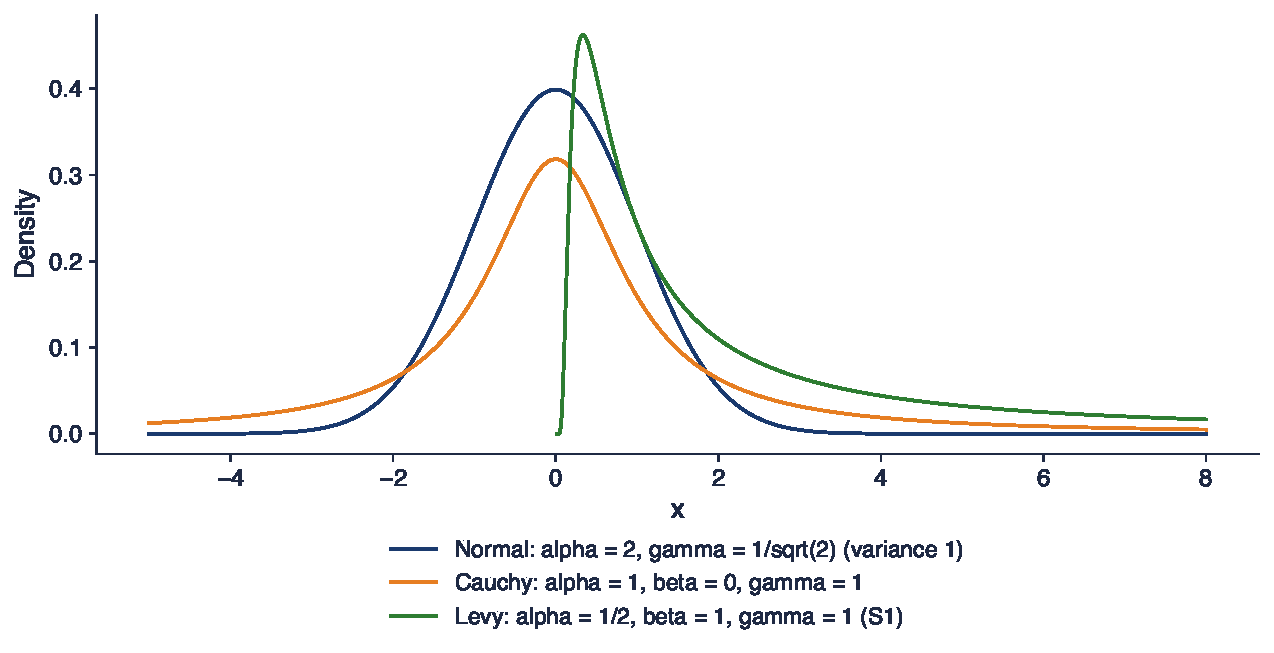
\includegraphics[width=0.97\textwidth,height=0.60\textheight,keepaspectratio]{sfm_ch3_special_cases.pdf}
\end{center}
\vspace{-0.25cm}
\begin{itemize}
    \item Cauchy: lower peak, much heavier tails than the Normal distribution with variance 1
    \item Lévy: only positive values, a long right tail; its mean is infinite
\end{itemize}
\quantlet{SFM\_ch3\_densities}{\qlurl{SFM_ch3_densities}}
\end{frame}

\begin{frame}{Worked Example: S1 vs S0 at $t = 1$}
\itemsize{\small}
\begin{itemize}
    \item $X$ with $\alpha = 1.5$, $\beta = 0.3$, $\gamma = 1$, $\delta = 0$; note $\tan\frac{3\pi}{4} = -1$
    \item \textbf{S1}: $\ln\varphi(1) = -1\cdot[1 - i \cdot 0.3 \cdot (-1)] = -1 - 0.3i$
    \begin{itemize}
        \item $\varphi(1) = e^{-1}(\cos 0.3 - i \sin 0.3) = 0.351 - 0.109i$; $|\varphi(1)| = e^{-1} = 0.368$
    \end{itemize}
    \item \textbf{S0}: the factor $|t|^{1-\alpha} - 1$ is 0 at $t = 1$, so $\varphi(1) = e^{-1} = 0.368$, a real number
    \begin{itemize}
        \item same modulus: the two laws differ only by a shift
        \item shift $= \beta\gamma\tan\frac{\pi\alpha}{2} = -0.3$: the S1 law with $\delta_1 = 0$ is the S0 law with $\delta_0 = -0.3$
    \end{itemize}
\end{itemize}
\end{frame}

\begin{frame}{Recap: Parameters and the Characteristic Function}
\itemsize{\small}
\begin{itemize}
    \item Stable laws are defined by $\varphi(t)$; the density is computed numerically
    \item $\alpha$ tails, $\beta$ skewness, $\gamma$ scale, $\delta$ location
    \item S0 vs S1: only $\delta$ differs, $\delta_0 = \delta_1 + \beta\gamma\tan\frac{\pi\alpha}{2}$; scipy uses S1 by default
    \item Closed forms: Normal ($\alpha = 2$, variance $2\gamma^2$), Cauchy, Lévy
\end{itemize}
\end{frame}


%=============================================================================
\section{Tails and Moments}
%=============================================================================

\begin{frame}{Power-Law Tails}
\itemsize{\small}
\begin{itemize}
    \item For $\alpha < 2$, as $x \to \infty$ \refNolan:
    \begin{itemize}
        \item $P(X > x) \sim \gamma^\alpha c_\alpha (1 + \beta)\, x^{-\alpha}$ and $P(X < -x) \sim \gamma^\alpha c_\alpha (1 - \beta)\, x^{-\alpha}$
        \item $c_\alpha = \Gamma(\alpha)\sin(\pi\alpha/2)/\pi$, with $\Gamma$ the gamma function; $f \sim g$ means $f/g \to 1$
    \end{itemize}
    \item On log-log axes the tail is a straight line with slope $-\alpha$
    \begin{itemize}
        \item doubling the threshold divides the tail probability by $2^\alpha$: $\times 0.31$ for $\alpha = 1.7$
    \end{itemize}
    \item The Normal tail falls like $e^{-x^2/(4\gamma^2)}$: doubling the threshold makes it vanish
    \item $\beta = \pm 1$ with $\alpha < 1$: one tail is missing (the law lives on a half-line)
\end{itemize}
\end{frame}

\begin{frame}{Tails on Log-Log Axes}
\itemsize{\footnotesize}
\begin{center}
    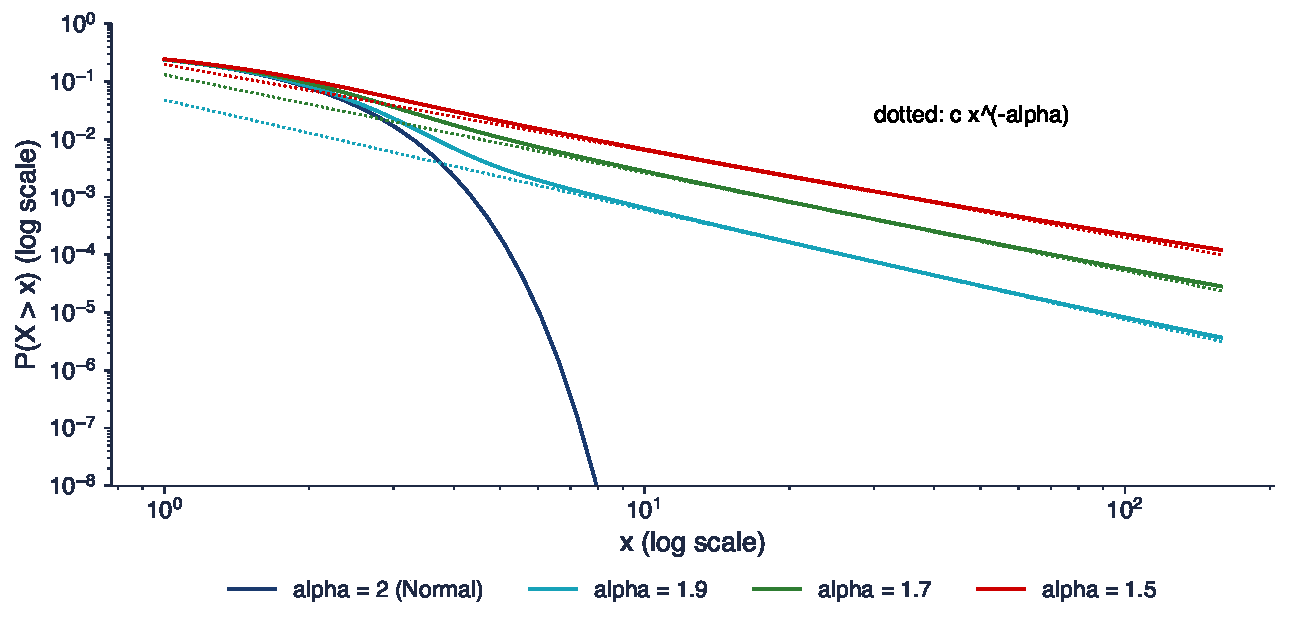
\includegraphics[width=0.97\textwidth,height=0.64\textheight,keepaspectratio]{sfm_ch3_tails_loglog.pdf}
\end{center}
\vspace{-0.25cm}
\begin{itemize}
    \item Solid: $P(X > x)$ of $S(\alpha, 0, 1, 0)$; dotted: the power law $c_\alpha x^{-\alpha}$, reached already near $x = 5$
    \item $P(X > 10)$: $0.279\%$ for $\alpha = 1.7$, $0.667\%$ for $\alpha = 1.5$, about $8\times 10^{-11}\%$ for the Normal distribution
\end{itemize}
\quantlet{SFM\_ch3\_tails\_moments}{\qlurl{SFM_ch3_tails_moments}}
\end{frame}

\begin{frame}{Which Moments Exist?}
\itemsize{\small}
\begin{itemize}
    \item For $0 < \alpha < 2$: $E|X|^p < \infty$ if and only if $p < \alpha$
    \begin{itemize}
        \item $E|X|^p$: the absolute moment of order $p > 0$; $p = 1$ gives the mean, $p = 2$ the variance
        \item reason: $|x|^p$ times a density of order $|x|^{-\alpha-1}$ is integrable only if $p < \alpha$
    \end{itemize}
    \item Consequences
    \begin{itemize}
        \item $\alpha < 2$: \textbf{infinite variance}; skewness and kurtosis are not defined
        \item $1 < \alpha < 2$: the mean exists; in S1 it equals $\delta_1$
        \item $\alpha \le 1$: not even the mean exists (Cauchy, Lévy)
        \item $\alpha = 2$: all moments exist
    \end{itemize}
    \item \textbf{What do you think?} Mandelbrot found $\alpha \approx 1.7$ for cotton. Does the mean daily change exist?
    \item \textbf{Answer}
    \begin{itemize}
        \item yes, because $1 < 1.7$; but the variance does not, because $2 > 1.7$
    \end{itemize}
\end{itemize}
\end{frame}

\begin{frame}{The Sample Variance Does Not Settle}
\itemsize{\footnotesize}
\begin{center}
    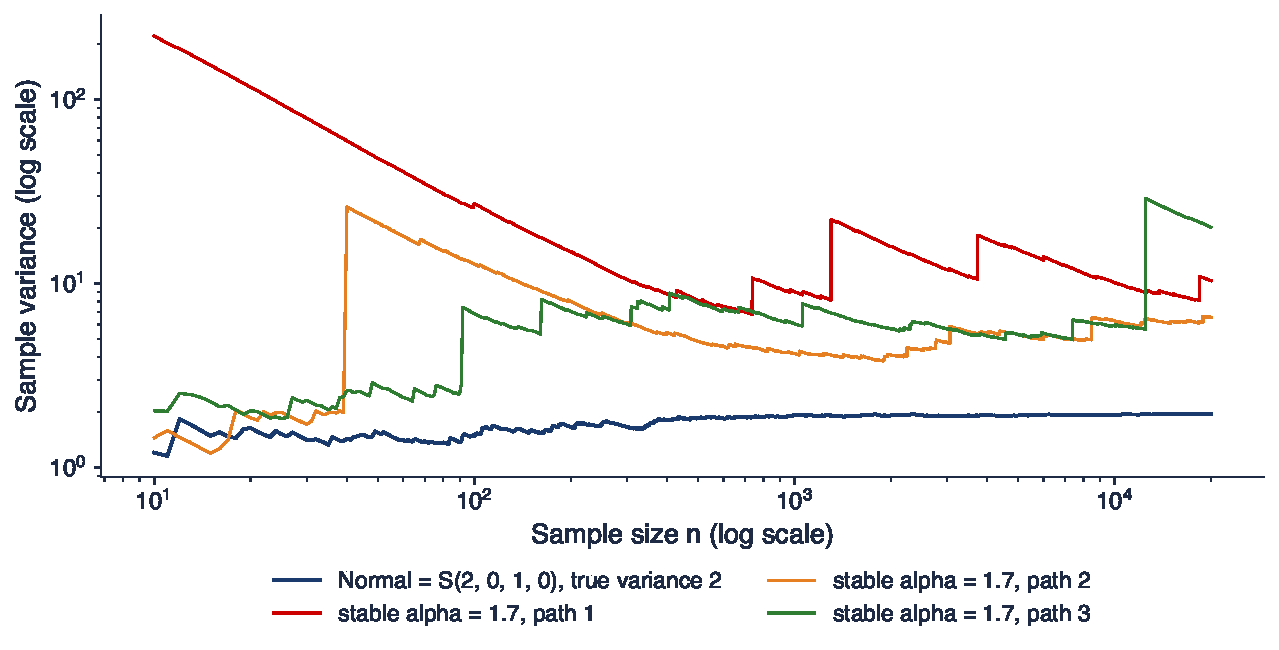
\includegraphics[width=0.97\textwidth,height=0.64\textheight,keepaspectratio]{sfm_ch3_running_var_sim.pdf}
\end{center}
\vspace{-0.25cm}
\begin{itemize}
    \item Normal (blue): the sample variance converges to the true value 2
    \item Stable $\alpha = 1.7$: each large draw makes the variance jump; after 20\,000 draws the three paths end at $10.4$, $6.6$, $20.2$
    \item Mandelbrot saw exactly this in cotton prices
\end{itemize}
\quantlet{SFM\_ch3\_tails\_moments}{\qlurl{SFM_ch3_tails_moments}}
\end{frame}

\begin{frame}{Tail Probabilities: Stable vs Normal}
\itemsize{\small}
\begin{center}
\footnotesize
\begin{tabular}{rrrr}
\toprule
$k$ & $P(|X| > k)$, Normal \% & $P(|X| > k)$, $\alpha = 1.7$ \% & ratio \\
\midrule
$2$ & $15.73$ & $18.59$ & $1.2$ \\
$3$ & $3.39$ & $7.25$ & $2.1$ \\
$5$ & $0.041$ & $2.13$ & $52.4$ \\
$10$ & $1.5\times 10^{-10}$ & $0.56$ & $3.6\times 10^{9}$ \\
\bottomrule
\end{tabular}
\end{center}
\begin{itemize}
    \item Both laws with $\beta = 0$, $\gamma = 1$, $\delta = 0$: the Normal law is $N(0, 2)$
    \item Near the centre the two laws are close; far in the tails they differ by orders of magnitude
    \item A risk model is judged in the tails, where the choice of law matters most
\end{itemize}\quantlet{SFM\_ch3\_tails\_moments}{\qlurl{SFM_ch3_tails_moments}}
\end{frame}

\begin{frame}{Infinite Variance and Risk Measures}
\itemsize{\small}
\begin{itemize}
    \item Tools that need a finite variance
    \begin{itemize}
        \item volatility, the Sharpe ratio and its standard error (\sfmchlink{https://danpele.github.io/SFM/EN/Courses/chapter1_data_returns_indicators.pdf}{Chapter 1}); mean--variance portfolios; confidence intervals based on the CLT
        \item with $\alpha < 2$ these numbers exist in every sample but estimate nothing
    \end{itemize}
    \item Tools that survive
    \begin{itemize}
        \item quantiles always exist: $\mathrm{VaR}_{1\%} = -q_{1\%}$, the loss exceeded with probability 1\%
        \item $\mathrm{ES}_{2.5\%}$ (expected shortfall, the mean loss beyond the VaR) exists only if $\alpha > 1$
        \item the scale $\gamma$ and the interquartile range replace the standard deviation
    \end{itemize}
    \item VaR and ES are developed in \sfmchlink{https://danpele.github.io/SFM/EN/Courses/chapter10_var_es_backtesting.pdf}{Chapter 10}
\end{itemize}
\end{frame}

\begin{frame}{Recap: Tails and Moments}
\itemsize{\small}
\begin{itemize}
    \item Tails: $P(|X| > x) \propto x^{-\alpha}$; a straight line on log-log axes
    \item Moments: $E|X|^p < \infty$ iff $p < \alpha$; $\alpha < 2$ means infinite variance
    \item The sample variance of a stable sample jumps and does not settle
    \item Quantiles, VaR and the scale $\gamma$ remain meaningful
\end{itemize}
\end{frame}


%=============================================================================
\section{Simulation}
%=============================================================================

\begin{frame}{The Chambers--Mallows--Stuck Method (Symmetric Case)}
\itemsize{\small}
\begin{itemize}
    \item No closed-form density, yet stable variables are easy to simulate \refCMS
    \item \textbf{CMS} (Chambers--Mallows--Stuck) for $S(\alpha, 0, 1, 0)$:
    \begin{itemize}
        \item draw $V \sim U(-\pi/2, \pi/2)$, a uniform angle, and $W \sim \mathrm{Exp}(1)$, an exponential variable with mean 1, independent
        \item $X = \dfrac{\sin(\alpha V)}{(\cos V)^{1/\alpha}} \left(\dfrac{\cos((1 - \alpha)V)}{W}\right)^{(1 - \alpha)/\alpha}$
        \item then $\gamma X + \delta \sim S(\alpha, 0, \gamma, \delta)$
    \end{itemize}
    \item Checks on special cases
    \begin{itemize}
        \item $\alpha = 1$: $X = \tan V$, a Cauchy variable
        \item $\alpha = 2$: $X = 2\sin V\sqrt{W}$, a $N(0, 2)$ variable
    \end{itemize}
\end{itemize}
\end{frame}

\begin{frame}{The General Case ($\beta \ne 0$)}
\itemsize{\small}
\begin{itemize}
    \item For $\alpha \ne 1$, S1 parameterisation \refWeron:
    \begin{itemize}
        \item $B = \dfrac{\arctan(\beta\tan\frac{\pi\alpha}{2})}{\alpha}$, \quad $S = \Big(1 + \beta^2\tan^2\frac{\pi\alpha}{2}\Big)^{1/(2\alpha)}$
        \item $X = S\,\dfrac{\sin(\alpha(V + B))}{(\cos V)^{1/\alpha}} \left(\dfrac{\cos(V - \alpha(V + B))}{W}\right)^{(1 - \alpha)/\alpha} \sim S(\alpha, \beta, 1, 0; 1)$
    \end{itemize}
    \item $B$, $S$: auxiliary constants that depend only on $\alpha$ and $\beta$; for $\beta = 0$, $B = 0$ and $S = 1$
    \item From the standard draw to any parameters
    \begin{itemize}
        \item S1: $\gamma X + \delta_1$; S0: $\gamma X + \delta_0 - \beta\gamma\tan\frac{\pi\alpha}{2}$
    \end{itemize}
    \item Weron (1996) corrected a formula of the original paper for $\beta \ne 0$; \texttt{scipy.stats.levy\_stable.rvs} uses the same method
\end{itemize}
\end{frame}

\begin{frame}{Worked Example: One Draw Step by Step}
\itemsize{\small}
\begin{itemize}
    \item $\alpha = 1.5$, $\beta = 0$; a uniform draw $U = 0.8$ and an exponential draw $W = 1.2$
    \item Steps
    \begin{itemize}
        \item $V = \pi(U - 1/2) = 0.942$: turns $U$, uniform on $(0, 1)$, into a uniform angle on $(-\pi/2, \pi/2)$
        \item $\sin(\alpha V) = 0.988$; $(\cos V)^{1/\alpha} = 0.702$
        \item $\big(\cos((1 - \alpha)V)/W\big)^{(1 - \alpha)/\alpha} = 1.104$
        \item $X = 0.988/0.702 \times 1.104 = 1.554$
    \end{itemize}
    \item Repeat with new $(U, W)$ pairs to obtain a sample of any size
\end{itemize}
\end{frame}

\begin{frame}{CMS Draws against the Exact Density}
\itemsize{\footnotesize}
\begin{center}
    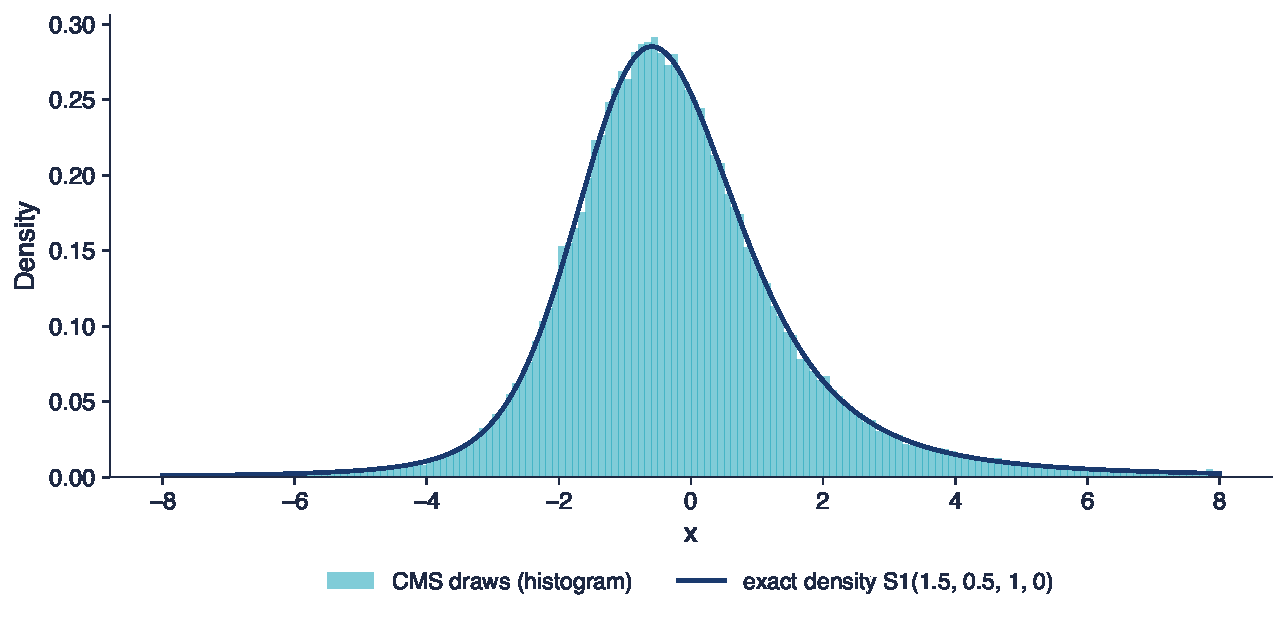
\includegraphics[width=0.97\textwidth,height=0.64\textheight,keepaspectratio]{sfm_ch3_cms.pdf}
\end{center}
\vspace{-0.25cm}
\begin{itemize}
    \item 100\,000 CMS draws of $S(1.5, 0.5, 1, 0; 1)$: the histogram follows the density computed from $\varphi$
    \item Quantiles 1\% and 99\%: sample $-5.47$ and $9.52$, exact $-5.40$ and $9.76$
    \item Two-sample KS (Kolmogorov--Smirnov) test against \texttt{levy\_stable.rvs}: statistic $0.0044$, p-value $0.30$, no difference
\end{itemize}
\quantlet{SFM\_ch3\_sim\_stable}{\qlurl{SFM_ch3_sim_stable}}
\end{frame}

\begin{frame}{Recap: Simulation}
\itemsize{\small}
\begin{itemize}
    \item CMS: a uniform angle $V$ and an exponential $W$ give one stable draw
    \item Special cases check the formula: $\tan V$ (Cauchy), $2\sin V\sqrt{W}$ (Normal)
    \item Skewed case: the formula of \refWeron; shift by $\beta\gamma\tan\frac{\pi\alpha}{2}$ for S0
\end{itemize}
\end{frame}


%=============================================================================
\section{Estimation}
%=============================================================================

\begin{frame}{Three Families of Estimators}
\itemsize{\small}
\begin{itemize}
    \item \textbf{Quantile methods}: match sample quantiles to those of the stable law
    \begin{itemize}
        \item \refFamaRollB\ for symmetric laws; \refMcCulloch\ for all four parameters
    \end{itemize}
    \item \textbf{Characteristic-function methods}: regress the empirical $\ln(-\ln|\hat\varphi(t)|^2)$ on $\ln|t|$
    \begin{itemize}
        \item $\hat\varphi(t) = \frac1n\sum_{j=1}^n e^{itr_j}$: the empirical characteristic function; $|\varphi(t)|^2 = e^{-2\gamma^\alpha|t|^\alpha}$, so the log-log relation is linear in $\ln|t|$
        \item \refKoutrouvelis; the slope estimates $\alpha$
    \end{itemize}
    \item \textbf{Maximum likelihood} (ML): the most precise, once the density can be computed
    \begin{itemize}
        \item \refNolanML, \refMRDC
    \end{itemize}
    \item A SAS implementation of these estimators is described in \refPele
\end{itemize}
\end{frame}

\begin{frame}{McCulloch's Quantile Method}
\itemsize{\small}
\begin{itemize}
    \item Two ratios of sample quantiles $\hat q_p$, free of location and scale \refMcCulloch:
    \begin{itemize}
        \item $\nu_\alpha = \dfrac{\hat q_{0.95} - \hat q_{0.05}}{\hat q_{0.75} - \hat q_{0.25}}$ (tail width relative to the body)
        \item $\nu_\beta = \dfrac{\hat q_{0.95} + \hat q_{0.05} - 2\hat q_{0.5}}{\hat q_{0.95} - \hat q_{0.05}}$ (asymmetry)
    \end{itemize}
    \item $\hat q_p$: the sample quantile of order $p$, the value below which a share $p$ of the returns lies
    \item Tables III and IV of the paper map $(\nu_\alpha, \nu_\beta)$ to $(\hat\alpha, \hat\beta)$
    \begin{itemize}
        \item Normal distribution: $\nu_\alpha = 2.439$; larger $\nu_\alpha$ means smaller $\alpha$
    \end{itemize}
    \item Then $\hat\gamma = (\hat q_{0.75} - \hat q_{0.25})/\phi_3(\hat\alpha, \hat\beta)$ (Table V) and $\hat\delta_0$ from Table VII; $\phi_3$: the interquartile range of $S(\alpha, \beta, 1, 0)$
    \item Fast, consistent, valid for $0.6 \le \alpha \le 2$; less precise than ML; a good starting point for ML
\end{itemize}
\end{frame}

\begin{frame}{McCulloch's Map from $\nu_\alpha$ to $\alpha$}
\itemsize{\footnotesize}
\begin{columns}[T]
\begin{column}{0.58\textwidth}
\begin{center}
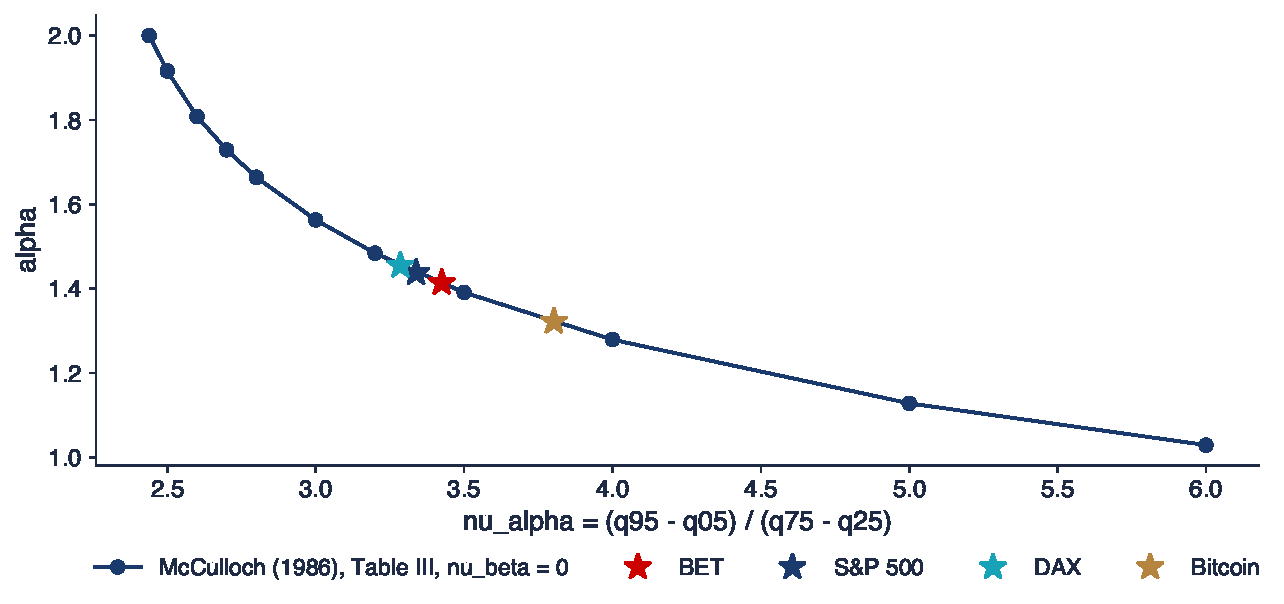
\includegraphics[width=\linewidth,height=0.78\textheight,keepaspectratio]{sfm_ch3_mcculloch_map.pdf}
\end{center}
\end{column}
\begin{column}{0.38\textwidth}
\begin{itemize}
    \item Line: Table III for a symmetric sample ($\nu_\beta = 0$)
    \item Stars: daily log returns since 2000 (Bitcoin since 2014)
    \item $\nu_\alpha$: BET $3.425$, S\&P 500 $3.338$, DAX $3.285$, Bitcoin $3.803$
    \item All well above 2.439: tails much wider than the Normal distribution allows
\end{itemize}
\end{column}
\end{columns}
\quantlet{SFM\_ch3\_estimation}{\qlurl{SFM_ch3_estimation}}
\end{frame}

\begin{frame}{Worked Example: McCulloch on the BET}
\itemsize{\small}
\begin{itemize}
    \item BET daily log returns (\%), 2000--2026, $n = 6\,670$
    \item Step 1: quantiles
    \begin{itemize}
        \item $\hat q_{0.05} = -1.93$, $\hat q_{0.25} = -0.50$, $\hat q_{0.5} = 0.08$, $\hat q_{0.75} = 0.66$, $\hat q_{0.95} = 2.06$
    \end{itemize}
    \item Step 2: ratios
    \begin{itemize}
        \item $\nu_\alpha = 4.00/1.17 = 3.425$; $\nu_\beta = -0.006$, practically symmetric
    \end{itemize}
    \item Step 3: Table III, column $\nu_\beta = 0$: $\nu_\alpha = 3.2 \mapsto 1.484$, $\nu_\alpha = 3.5 \mapsto 1.391$
    \begin{itemize}
        \item linear interpolation: $\hat\alpha \approx 1.414$
    \end{itemize}
    \item Step 4: $\hat\gamma = 0.60$ (\% a day), $\hat\beta = -0.011$, $\hat\delta_0 = 0.079$
\end{itemize}\quantlet{SFM\_ch3\_estimation}{\qlurl{SFM_ch3_estimation}}
\end{frame}

\begin{frame}{Maximum Likelihood}
\itemsize{\small}
\begin{itemize}
    \item Log-likelihood of a sample $r_1, \dots, r_n$: $\ell(\theta) = \sum_{t=1}^n \ln f(r_t; \theta)$, $\theta = (\alpha, \beta, \gamma, \delta_0)$
    \begin{itemize}
        \item $\theta$: the vector of the four parameters; $f(r_t; \theta)$: the stable density at $r_t$; $\hat\theta$ maximises $\ell$ numerically, starting from the McCulloch estimate
        \item standard errors from the curvature of $\ell$: the inverse of the Hessian, the matrix of second derivatives of $\ell$
    \end{itemize}
    \item The density $f$ is computed from $\varphi$
    \begin{itemize}
        \item $f(x) = \frac{1}{2\pi}\int e^{-itx}\varphi(t)\,dt$, evaluated on a grid with the FFT (fast Fourier transform) \refMDC
        \item or by direct integration \refNolanA; \texttt{levy\_stable.fit} does this and needs minutes for a few thousand returns
    \end{itemize}
    \item ML in S0 is regular for $\alpha \in (0, 2)$: standard errors shrink like $1/\sqrt{n}$ \refNolanML
\end{itemize}
\end{frame}

\begin{frame}{McCulloch vs ML in a Monte Carlo Study}
\itemsize{\footnotesize}
\begin{center}
    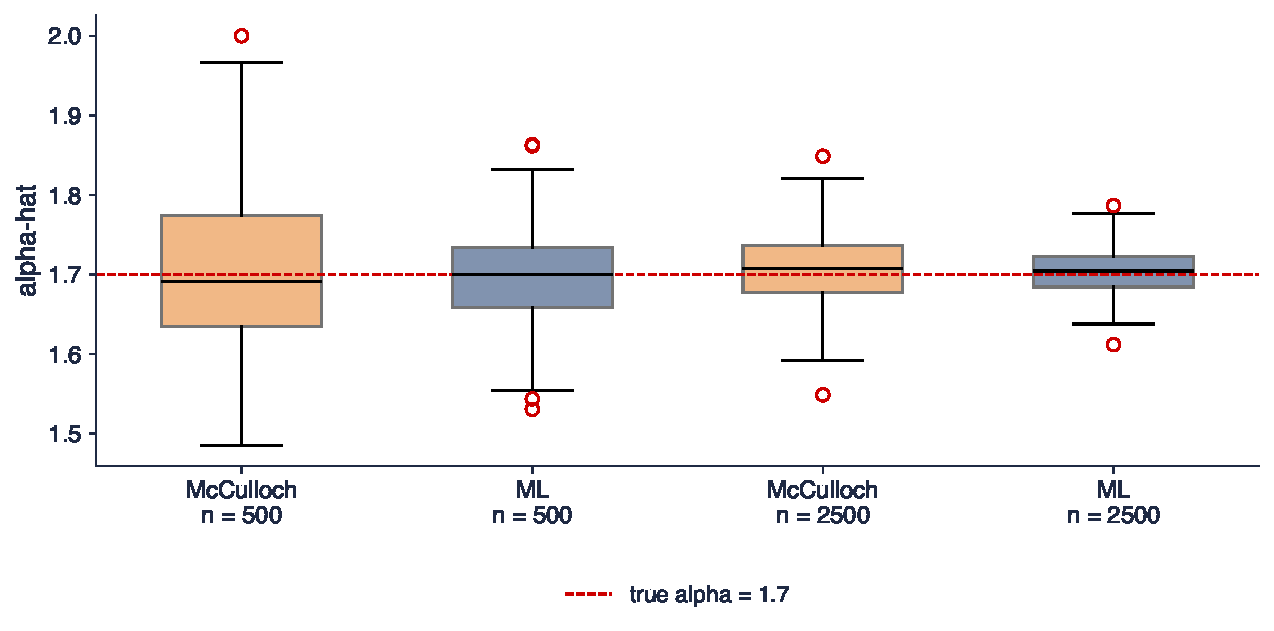
\includegraphics[width=0.97\textwidth,height=0.60\textheight,keepaspectratio]{sfm_ch3_estimators_mc.pdf}
\end{center}
\vspace{-0.25cm}
\begin{itemize}
    \item 200 samples of $S(1.7, 0, 1, 0)$ for each size; both estimators are centred on 1.7
    \item Standard deviation of $\hat\alpha$: $n = 500$: McCulloch $0.107$, ML $0.061$; $n = 2500$: $0.046$ vs $0.030$
    \item ML is about $1.7$ times more precise for the same data
\end{itemize}
\quantlet{SFM\_ch3\_estimation}{\qlurl{SFM_ch3_estimation}}
\end{frame}

\begin{frame}{Recap: Estimation}
\itemsize{\small}
\begin{itemize}
    \item McCulloch: five quantiles, two ratios, four tables; fast and robust
    \item ML: numerical density from $\varphi$, numerical maximisation; the most precise
    \item Report the parameterisation (S0 or S1) and the units of $\gamma$ and $\delta$
\end{itemize}
\end{frame}


%=============================================================================
\section{Fitting Real Returns}
%=============================================================================

\begin{frame}{Stable Fits of Daily Log Returns}
\itemsize{\small}
\begin{center}
\footnotesize
\begin{tabular}{lrrrrrrr}
\toprule
& $n$ & $\hat\alpha$ McC. & $\hat\alpha$ ML (SE) & $\hat\beta$ ML (SE) & $\hat\gamma$ & $\hat\delta_0$ & $\hat\delta_1$ \\
\midrule
BET & 6\,670 & $1.414$ & $1.486$ ($0.020$) & $-0.016$ ($0.034$) & $0.62$ & $0.088$ & $0.078$ \\
S\&P 500 & 6\,714 & $1.438$ & $1.540$ ($0.021$) & $-0.181$ ($0.036$) & $0.58$ & $0.093$ & $0.000$ \\
DAX & 6\,786 & $1.455$ & $1.606$ ($0.021$) & $-0.179$ ($0.040$) & $0.74$ & $0.090$ & $-0.004$ \\
Bitcoin & 4\,384 & $1.322$ & $1.410$ ($0.026$) & $0.019$ ($0.036$) & $1.54$ & $0.132$ & $0.171$ \\
\bottomrule
\end{tabular}
\end{center}
\begin{itemize}
    \item Daily log returns in \%; indices 2000--2026, Bitcoin 2014--2026 (7 days a week); data: EODHD
    \item McC.: McCulloch; ML in S0 with standard errors; $\hat\gamma$, $\hat\delta_0$, $\hat\delta_1$ in \% a day
\end{itemize}\quantlet{SFM\_ch3\_fit\_returns}{\qlurl{SFM_ch3_fit_returns}}
\end{frame}

\begin{frame}{Reading the Estimates}
\itemsize{\small}
\begin{itemize}
    \item $\hat\alpha$ well below 2 for all four series
    \begin{itemize}
        \item S\&P 500: $(2 - 1.540)/0.021 \approx 22$ standard errors from the Normal case
        \item the heaviest tails: Bitcoin ($\hat\alpha = 1.410$)
    \end{itemize}
    \item $\hat\beta < 0$ for the S\&P 500 and the DAX: the left tail is heavier (crashes)
    \begin{itemize}
        \item BET and Bitcoin: $\hat\beta$ within two standard errors of 0
    \end{itemize}
    \item $\hat\gamma$: Bitcoin $1.54\%$ vs S\&P 500 $0.58\%$ a day; compare the sample standard deviations $3.49\%$ and $1.21\%$
    \item McCulloch gives lower $\hat\alpha$ than ML for every series: the two methods weigh the tails differently
\end{itemize}
\end{frame}

\begin{frame}{Fitted Densities on a Log Scale}
\itemsize{\footnotesize}
\begin{center}
    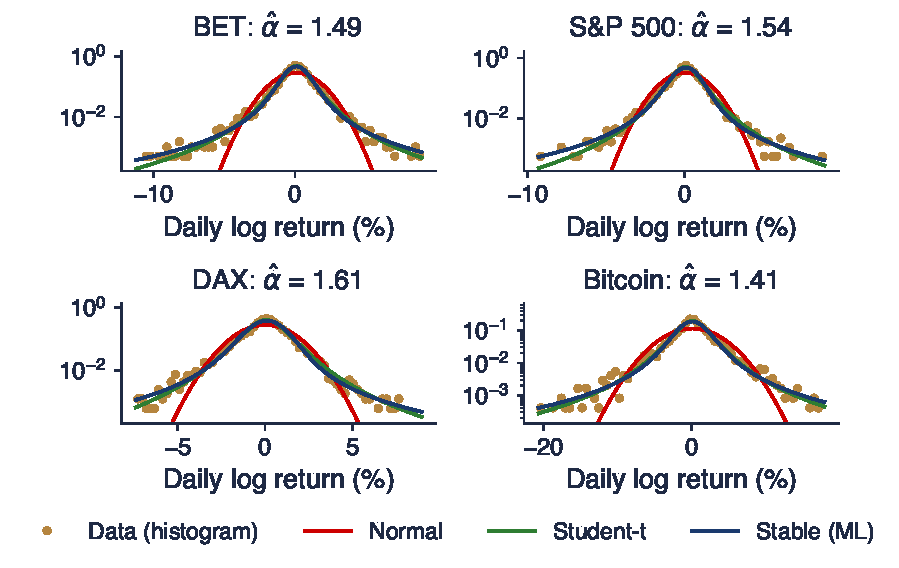
\includegraphics[width=0.97\textwidth,height=0.66\textheight,keepaspectratio]{sfm_ch3_fit_density.pdf}
\end{center}
\vspace{-0.25cm}
\begin{itemize}
    \item Normal (red): far too few large returns; Student-t (green) and stable (blue) both follow the body
    \item Far tails: the stable density stays above the data points; the Student-t is closer
\end{itemize}
\quantlet{SFM\_ch3\_fit\_returns}{\qlurl{SFM_ch3_fit_returns}}
\end{frame}

\begin{frame}{QQ Plots against the Three Models}
\itemsize{\footnotesize}
\begin{center}
    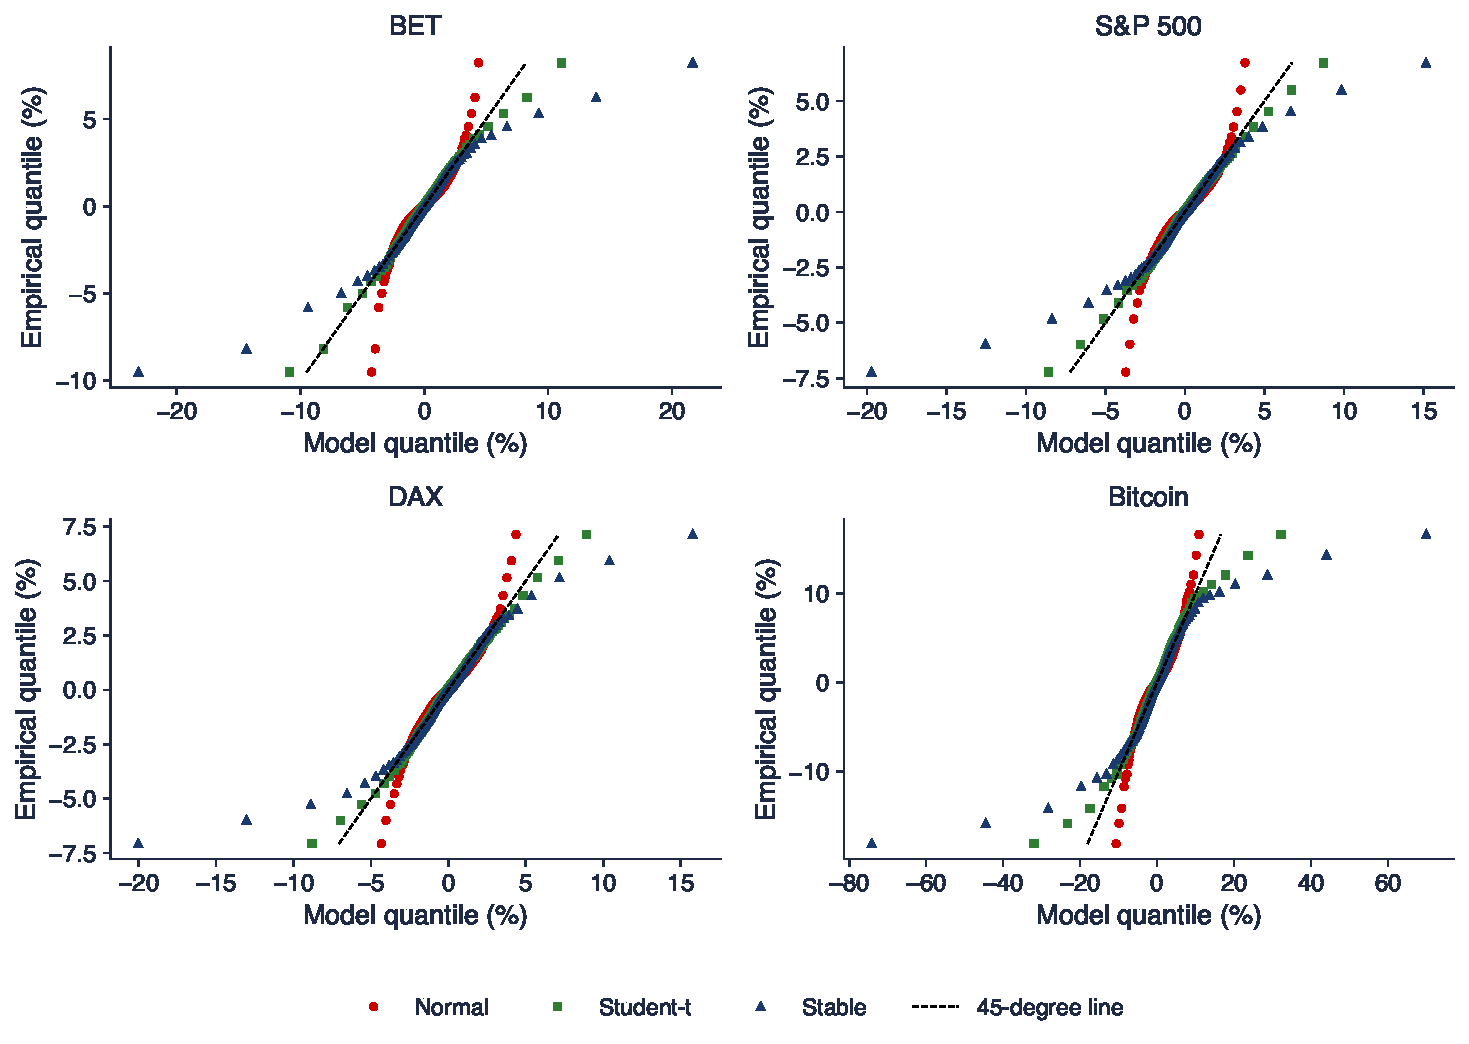
\includegraphics[width=0.97\textwidth,height=0.62\textheight,keepaspectratio]{sfm_ch3_qq_real.pdf}
\end{center}
\vspace{-0.25cm}
\begin{itemize}
    \item A QQ (quantile--quantile) plot puts the empirical quantiles against the model quantiles; a good model lies on the 45-degree line
    \item Normal: too-short tails (steep ends); stable: too-long tails (flat ends, model quantiles far beyond the data); Student-t: the closest
\end{itemize}
\quantlet{SFM\_ch3\_fit\_returns}{\qlurl{SFM_ch3_fit_returns}}
\end{frame}

\begin{frame}{The Left Tail on Log-Log Axes}
\itemsize{\footnotesize}
\begin{center}
    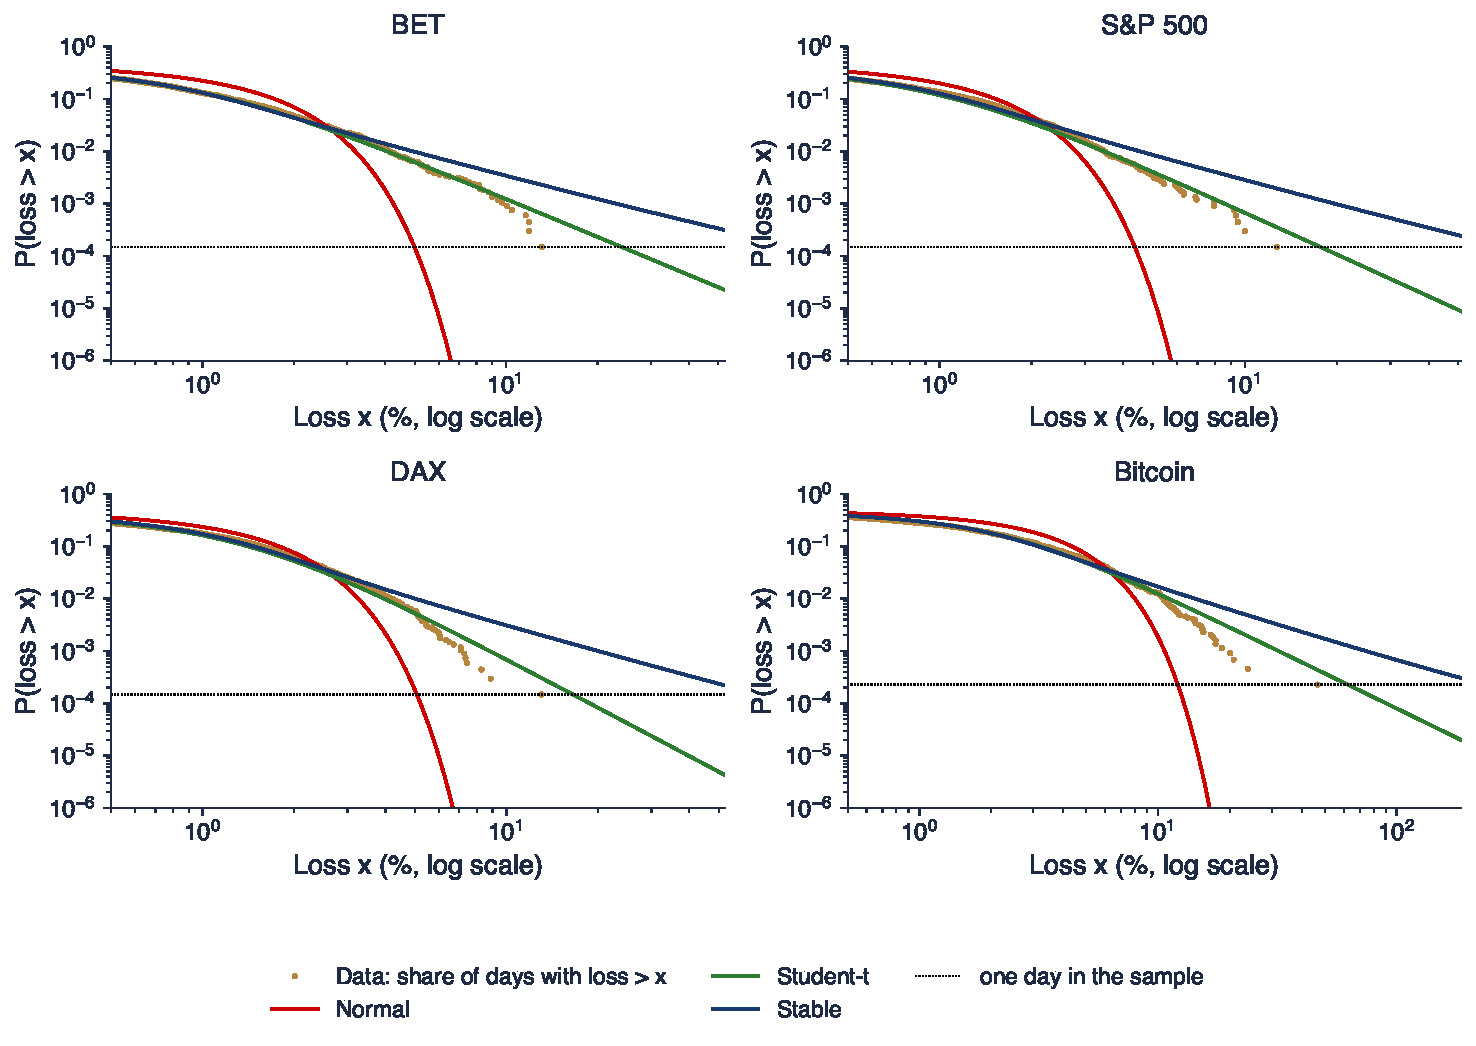
\includegraphics[width=0.97\textwidth,height=0.66\textheight,keepaspectratio]{sfm_ch3_tails_real.pdf}
\end{center}
\vspace{-0.25cm}
\begin{itemize}
    \item Points: share of days with a loss above $x$; lines: the same probability under each fitted model
    \item The empirical tail bends down faster than the stable line: the tail index of the data is larger than $\hat\alpha$
\end{itemize}
\quantlet{SFM\_ch3\_fit\_returns}{\qlurl{SFM_ch3_fit_returns}}
\end{frame}

\begin{frame}{Counting Large Losses}
\itemsize{\small}
\begin{center}
\footnotesize
\begin{tabular}{lrrrrr}
\toprule
& loss above & observed & Normal & Student-t & stable \\
\midrule
S\&P 500 & $5\%$ & 23 & $0.1$ & $27.0$ & $57.3$ \\
S\&P 500 & $10\%$ & 1 & $\approx 0$ & $4.5$ & $19.1$ \\
S\&P 500 & $15\%$ & 0 & $\approx 0$ & $1.5$ & $10.2$ \\
BET & $10\%$ & 6 & $\approx 0$ & $8.2$ & $22.8$ \\
Bitcoin & $10\%$ & 56 & $8.1$ & $54.2$ & $73.9$ \\
Bitcoin & $20\%$ & 4 & $\approx 0$ & $12.3$ & $26.9$ \\
\bottomrule
\end{tabular}
\end{center}
\begin{itemize}
    \item Expected number of days $= n \times P(r < -x)$ under each fitted model
    \item Normal: almost no large losses; stable: too many, and the gap grows with the threshold; Student-t: closest to the counts
    \item S\&P 500: 1 day below $-10\%$ in 6\,714 days; the stable fit expects $19.1$
\end{itemize}\quantlet{SFM\_ch3\_fit\_returns}{\qlurl{SFM_ch3_fit_returns}}
\end{frame}

\begin{frame}{VaR 1\% and VaR 0.1\% under the Three Models}
\itemsize{\small}
\begin{center}
\footnotesize
\begin{tabular}{l|rrrr|rrrr}
\toprule
& \multicolumn{4}{c|}{VaR 1\% (\%)} & \multicolumn{4}{c}{VaR 0.1\% (\%)} \\ & data & Normal & t & stable & data & Normal & t & stable \\
\midrule
BET & $4.1$ & $3.2$ & $4.1$ & $4.9$ & $9.5$ & $4.3$ & $10.9$ & $23.1$ \\
S\&P 500 & $3.5$ & $2.8$ & $3.5$ & $4.5$ & $7.2$ & $3.7$ & $8.6$ & $19.7$ \\
DAX & $4.2$ & $3.3$ & $4.0$ & $5.0$ & $7.1$ & $4.3$ & $8.8$ & $20.0$ \\
Bitcoin & $10.5$ & $8.0$ & $11.1$ & $14.3$ & $18.1$ & $10.7$ & $31.9$ & $74.2$ \\
\bottomrule
\end{tabular}
\end{center}
\begin{itemize}
    \item VaR at level $p$: $\mathrm{VaR}_p = -q_p$, the daily loss exceeded with probability $p$ (\sfmchlink{https://danpele.github.io/SFM/EN/Courses/chapter10_var_es_backtesting.pdf}{Chapter 10}); here $p$, because $\alpha$ is the stable index
    \item VaR 1\%: the Normal model is too low, the stable model too high
    \item VaR 0.1\%: the stable model gives roughly two to four times the empirical quantile
\end{itemize}\quantlet{SFM\_ch3\_fit\_returns}{\qlurl{SFM_ch3_fit_returns}}
\end{frame}

\begin{frame}{Which Model Fits Best?}
\itemsize{\small}
\begin{center}
\footnotesize
\begin{tabular}{lrrrr}
\toprule
& AIC Normal & AIC Student-t & AIC stable & $\hat\nu$ (Student-t) \\
\midrule
BET & 23\,407 & 20\,996 & 21\,088 & $2.43$ \\
S\&P 500 & 21\,650 & 19\,702 & 19\,794 & $2.67$ \\
DAX & 23\,901 & 22\,595 & 22\,697 & $3.09$ \\
Bitcoin & 23\,391 & 22\,056 & 22\,159 & $2.23$ \\
\bottomrule
\end{tabular}
\end{center}
\begin{itemize}
    \item AIC (Akaike information criterion) $= 2k - 2\ell(\hat\theta)$, with $k$ the number of parameters; lower is better
    \item Both heavy-tailed models beat the Normal distribution by thousands of AIC points
    \item Student-t wins for every series, with fewer parameters; S\&P 500: by 92 points
    \item $\hat\nu$ between 2 and 3.1: finite variance, but few finite moments beyond it
\end{itemize}\quantlet{SFM\_ch3\_fit\_returns}{\qlurl{SFM_ch3_fit_returns}}
\end{frame}

\begin{frame}{Recap: Fitting Real Returns}
\itemsize{\small}
\begin{itemize}
    \item All four series: $\hat\alpha$ between 1.410 and 1.606, far from 2
    \item The stable law fits the body much better than the Normal distribution
    \item It overstates the far tails: too many extreme losses, VaR 0.1\% too high
    \item By AIC, the Student-t distribution fits better
\end{itemize}
\end{frame}


%=============================================================================
\section{The Critique: Finite or Infinite Variance?}
%=============================================================================

\begin{frame}{Test 1: Does $\alpha$ Stay the Same When Returns Are Summed?}
\itemsize{\footnotesize}
\begin{center}
    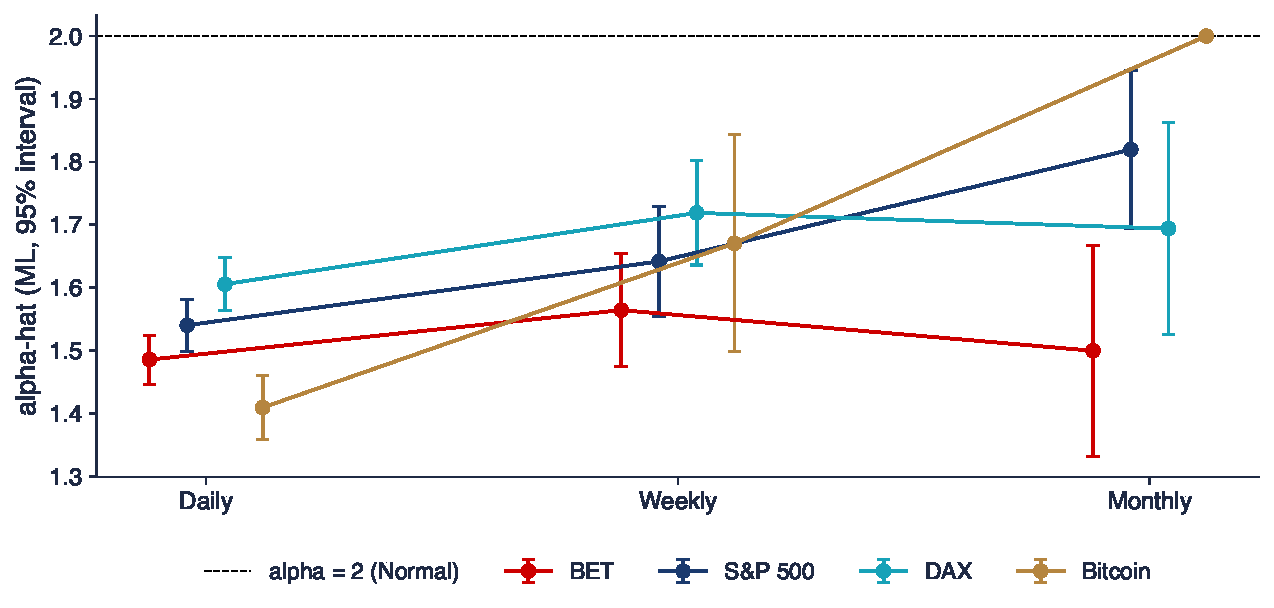
\includegraphics[width=0.97\textwidth,height=0.64\textheight,keepaspectratio]{sfm_ch3_aggregation.pdf}
\end{center}
\vspace{-0.25cm}
\begin{itemize}
    \item If daily returns were i.i.d.\ stable, weekly and monthly sums would have the \textbf{same} $\alpha$ (stability)
    \item ML estimates: S\&P 500 $1.54 \to 1.64 \to 1.82$; Bitcoin $1.41 \to 1.67 \to 2.00$ (at the bound 2)
\end{itemize}
\quantlet{SFM\_ch3\_aggregation}{\qlurl{SFM_ch3_aggregation}}
\end{frame}

\begin{frame}{Reading the Aggregation Test}
\itemsize{\small}
\begin{itemize}
    \item $\hat\alpha$ rises with the horizon for the S\&P 500, DAX and Bitcoin
    \begin{itemize}
        \item DAX: $1.61 \to 1.72 \to 1.69$; the daily and monthly intervals do not overlap for the S\&P 500
    \end{itemize}
    \item BET: $1.49 \to 1.56 \to 1.50$, no clear rise
    \begin{itemize}
        \item monthly samples are short (321 months): wide intervals
    \end{itemize}
    \item The same pattern in the classic studies: \refOfficer, \refAB
    \item A rising $\alpha$ is what the GCLT predicts for sums of finite-variance returns that converge slowly to the Normal distribution
\end{itemize}
\end{frame}

\begin{frame}{Test 2: Does the Sample Variance Settle?}
\itemsize{\footnotesize}
\begin{center}
    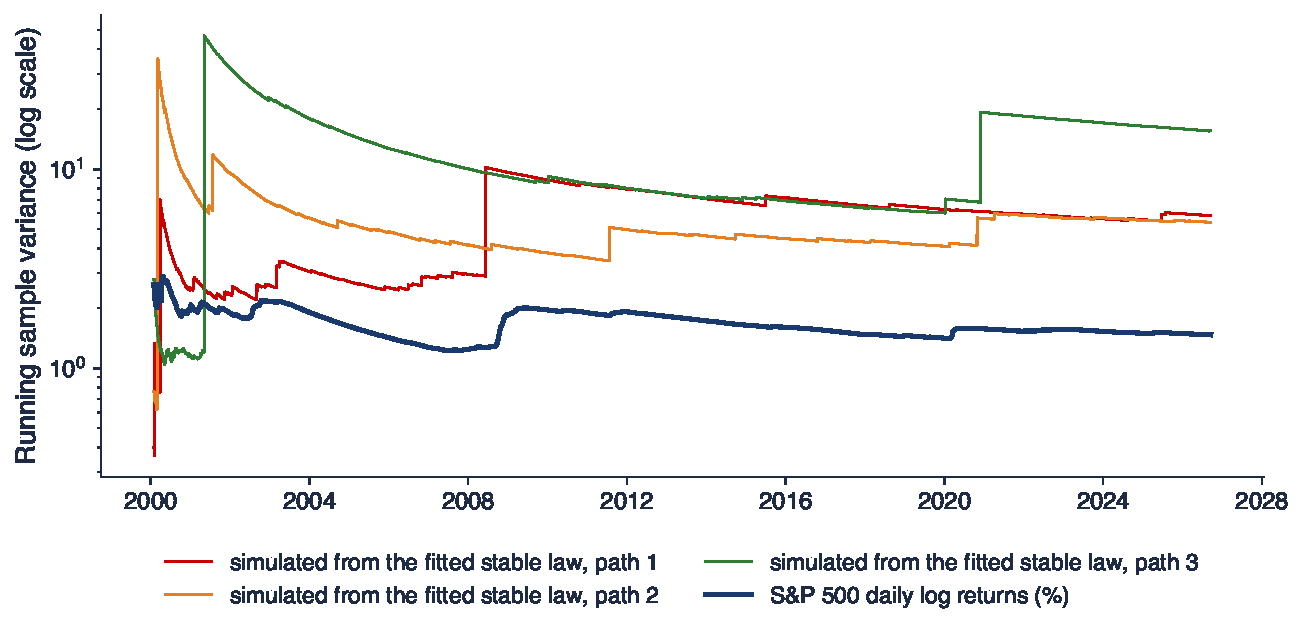
\includegraphics[width=0.97\textwidth,height=0.64\textheight,keepaspectratio]{sfm_ch3_running_var_real.pdf}
\end{center}
\vspace{-0.25cm}
\begin{itemize}
    \item S\&P 500 (blue): after the jumps of 2008 and 2020 the running variance settles near $1.47$
    \item Paths simulated from the fitted stable law, same length: final variances between $5.4$ and $15.6$, far above the data
\end{itemize}
\quantlet{SFM\_ch3\_aggregation}{\qlurl{SFM_ch3_aggregation}}
\end{frame}

\begin{frame}{Test 3: How Heavy Is the Far Tail?}
\itemsize{\small}
\begin{itemize}
    \item The stable $\alpha$ is driven by the whole distribution, mostly by the body
    \begin{itemize}
        \item the tail index of the far tail alone is estimated with the Hill estimator \refHill\ (\sfmchlink{https://danpele.github.io/SFM/EN/Courses/chapter5_heavy_tails_evt.pdf}{Chapter 5})
    \end{itemize}
    \item For stock indices the far tail decays roughly like $x^{-3}$, the ``inverse cubic law'' \refGopi
    \begin{itemize}
        \item a tail index near 3 means finite variance, and no stable law has it
    \end{itemize}
    \item Our counts agree: the stable fits expect many more losses beyond $10\%$ than observed
    \item \refLLW: further evidence against the stable model from the behaviour of sample moments
\end{itemize}
\end{frame}

\begin{frame}{Why Do Daily Returns Look Stable?}
\itemsize{\small}
\begin{itemize}
    \item \textbf{Volatility clustering} (\sfmchlink{https://danpele.github.io/SFM/EN/Courses/chapter2_classical_distributions_stylised_facts.pdf}{Chapters 2} and \sfmchlink{https://danpele.github.io/SFM/EN/Courses/chapter9_arch_garch_models.pdf}{9}): calm and turbulent periods alternate
    \begin{itemize}
        \item a mixture of Normal laws with changing variance has heavy tails and a finite variance \refBG
        \item fitted to one stable law, the mixture gives $\hat\alpha < 2$
    \end{itemize}
    \item \textbf{Truncated and tempered stable laws}: stable at moderate scales, lighter tails far out
    \begin{itemize}
        \item \refMS\ fitted a truncated Lévy flight to the S\&P 500
        \item \refGS: such laws explain why returns look stable at short horizons and Normal at long ones
    \end{itemize}
\end{itemize}
\end{frame}

\begin{frame}{Verdict}
\itemsize{\small}
\begin{itemize}
    \item \textbf{Mandelbrot was right} about the facts
    \begin{itemize}
        \item daily returns have heavy tails; the Normal distribution fails badly
    \end{itemize}
    \item \textbf{The infinite variance is not supported}
    \begin{itemize}
        \item $\hat\alpha$ rises with aggregation; the sample variance settles; the far tail is lighter than any stable tail
    \end{itemize}
    \item Where stable laws remain useful
    \begin{itemize}
        \item a benchmark for heavy tails; simulation; the scaling idea; data with truly infinite variance (some insurance losses, some crypto tokens)
        \item the GCLT: a reminder that $\sqrt{n}$-rules need a finite variance
    \end{itemize}
    \item Next: \sfmchlink{https://danpele.github.io/SFM/EN/Courses/chapter5_heavy_tails_evt.pdf}{Chapter 5} estimates the tail index directly with extreme value theory
\end{itemize}
\end{frame}

\begin{frame}{Recap: The Critique}
\itemsize{\small}
\begin{itemize}
    \item Stability predicts the same $\alpha$ at every horizon: the data show a rising $\alpha$
    \item The sample variance of real returns settles; that of stable samples does not
    \item Volatility clustering and tempered tails explain the apparent $\alpha < 2$
    \item Heavy tails: yes; infinite variance: no
\end{itemize}
\end{frame}


%=============================================================================
\section{AI for Scientific Discovery}
%=============================================================================

\begin{frame}{An Open Question}
\itemsize{\small}
\begin{itemize}
    \item \textbf{Have the tails of Bitcoin become lighter as the market matured?}
    \begin{itemize}
        \item more participants, futures and ETFs (exchange-traded funds) since 2017--2024
        \item if the tails got lighter, risk models fitted on old data overstate today's risk
    \end{itemize}
    \item Why it is open: $\hat\alpha$ moves with volatility regimes, and yearly samples are short
    \item Full sample: $\hat\alpha = 1.410$ (SE $0.026$), the lowest of our four series
    \item AI tools can speed up such a study; they do not replace checking it \refWang
\end{itemize}
\end{frame}

\begin{frame}{How AI Could Help}
\itemsize{\small}
\begin{itemize}
    \item \textbf{Literature}: list papers on tail estimates for crypto assets and summarise their methods
    \item \textbf{Code}: draft a rolling-window McCulloch estimator with bootstrap intervals
    \item \textbf{Robustness}: propose other windows, ML instead of quantiles, Student-t $\nu$ instead of $\alpha$
    \item \textbf{Explanation}: a first draft of the interpretation of a table of yearly estimates
    \item Example prompt
    \begin{itemize}
        \item \aiprompt{Write a Python function that estimates the stable alpha of daily log returns on rolling 365-day windows with McCulloch (1986), and adds 95\% bootstrap intervals.}
    \end{itemize}
\end{itemize}
\end{frame}

\begin{frame}{What to Check}
\itemsize{\small}
\begin{itemize}
    \item Parameterisation: S0 or S1; scipy uses S1 by default; the location differs by $\beta\gamma\tan\frac{\pi\alpha}{2}$
    \item Units: returns in \% or in decimals; $\gamma$ and $\delta$ change, $\alpha$ and $\beta$ do not
    \item Overlapping windows are not independent: do not read the rolling estimates as separate tests
    \item Numbers: recompute one window with a second method (ML or the quantile tables)
    \item References: every cited paper must exist; check the DOI
\end{itemize}
\end{frame}

\begin{frame}{Project Seed}
\itemsize{\small}
\begin{itemize}
    \item \textbf{Question}: is the tail of Bitcoin returns lighter now than in 2014--2018?
    \begin{itemize}
        \item data: Bitcoin daily closes from the course data (EODHD), 2014--2026
    \end{itemize}
    \item Steps
    \begin{itemize}
        \item estimate $\alpha$ by McCulloch and by ML for each calendar year, with bootstrap intervals
        \item repeat on returns divided by a rolling volatility: does the trend survive?
        \item compare with the Student-t $\hat\nu$ of each year
    \end{itemize}
    \item Deliverable: one table, one chart, and a paragraph on what the data can and cannot show
    \item Declare any AI use, and list the errors of the AI that you corrected
\end{itemize}
\end{frame}


%=============================================================================
\section{Summary}
%=============================================================================

\begin{frame}{Key Takeaways}
\itemsize{\small}
\begin{itemize}
    \item Stable laws are the only laws whose sums keep the same shape, and the only limits of normalised sums (GCLT)
    \item Four parameters: $\alpha$ tails, $\beta$ skewness, $\gamma$ scale, $\delta$ location; know your parameterisation (S0 or S1)
    \item $\alpha < 2$: power-law tails and infinite variance; $\alpha \le 1$: no mean
    \item Simulate with CMS; estimate with McCulloch quantiles or ML
    \item Daily returns: $\hat\alpha \approx 1.4$--$1.6$, much better than the Normal distribution in the body
    \item But $\hat\alpha$ rises with aggregation and the variance settles: heavy tails, finite variance
\end{itemize}
\end{frame}

\begin{frame}{Key Formulas}
\itemsize{\small}
{\renewcommand{\arraystretch}{1.45}\begin{center}
\scriptsize
\begin{tabular}{ll}
\toprule
\textbf{Quantity} & \textbf{Formula} \\
\midrule
Stability & $aX_1 + bX_2 \overset{d}{=} cX + d$, \quad $c^\alpha = a^\alpha + b^\alpha$ \\
Sum of $n$ copies & $X_1 + \dots + X_n \overset{d}{=} n^{1/\alpha}X + d_n$ \\
Characteristic function (S1) & $\exp\{-\gamma^\alpha|t|^\alpha[1 - i\beta\,\mathrm{sign}(t)\tan\frac{\pi\alpha}{2}] + i\delta_1 t\}$ \\
S0 vs S1 & $\delta_0 = \delta_1 + \beta\gamma\tan\frac{\pi\alpha}{2}$ \\
Normal case & $S(2, \beta, \gamma, \delta) = N(\delta, 2\gamma^2)$ \\
Tails & $P(X > x) \sim \gamma^\alpha c_\alpha(1 + \beta)x^{-\alpha}$ \\
Moments & $E|X|^p < \infty \iff p < \alpha$ \quad ($\alpha < 2$) \\
CMS ($\beta = 0$) & $\dfrac{\sin(\alpha V)}{(\cos V)^{1/\alpha}}\Big(\dfrac{\cos((1-\alpha)V)}{W}\Big)^{(1-\alpha)/\alpha}$ \\
McCulloch & $\nu_\alpha = \dfrac{q_{0.95} - q_{0.05}}{q_{0.75} - q_{0.25}}$, \quad $\nu_\beta = \dfrac{q_{0.95} + q_{0.05} - 2q_{0.5}}{q_{0.95} - q_{0.05}}$ \\
\bottomrule
\end{tabular}
\end{center}
}
\end{frame}

\begin{frame}{Check Yourself}
\itemsize{\small}
\begin{itemize}
    \item \textbf{Question}: daily returns are i.i.d.\ $S(1.5, 0, \gamma, 0)$; by what factor does the scale grow from 1 day to 20 days?
    \begin{itemize}
        \item \textbf{Answer}: $20^{1/1.5} = 7.37$, i.e.\ $1.65$ times the square-root-of-time factor $\sqrt{20}$
    \end{itemize}
    \item \textbf{Question}: a fitted law has $\alpha = 1.2$; do the mean and the variance exist?
    \begin{itemize}
        \item \textbf{Answer}: the mean exists ($1 < 1.2$), the variance does not ($2 > 1.2$)
    \end{itemize}
    \item \textbf{Question}: scipy reports $\delta = 0.05$ with $\alpha = 1.7$, $\beta = -0.2$, $\gamma = 0.6$; what is $\delta_0$?
    \begin{itemize}
        \item \textbf{Answer}: scipy uses S1, so $\delta_0 = 0.05 + (-0.2)(0.6)\tan(0.85\pi) = 0.05 + 0.061 = 0.111$
    \end{itemize}
    \item Next: \sfmchlink{https://danpele.github.io/SFM/EN/Courses/chapter4_probability.pdf}{Chapter 4}, probability for finance
\end{itemize}
\end{frame}


%=============================================================================
\section{References}
%=============================================================================

\begin{frame}{References (1/2)}
\itemsize{\tiny}
\begin{itemize}
    \item Akgiray, V., Booth, G.G. (1988). \href{https://doi.org/10.1080/07350015.1988.10509636}{The stable-law model of stock returns}. \textit{Journal of Business \& Economic Statistics}, 6(1), 51--57.
    \item Blattberg, R.C., Gonedes, N.J. (1974). \href{https://doi.org/10.1086/295634}{A comparison of the stable and Student distributions as statistical models for stock prices}. \textit{Journal of Business}, 47(2), 244--280.
    \item Borak, S., Härdle, W., Weron, R. (2005). \href{https://doi.org/10.1007/3-540-27395-6_1}{Stable distributions}. In Čížek, P., Härdle, W., Weron, R. (eds.), \textit{Statistical Tools for Finance and Insurance}, 21--44. Springer.
    \item Borak, S., Misiorek, A., Weron, R. (2011). \href{https://doi.org/10.1007/978-3-642-18062-0_1}{Models for heavy-tailed asset returns}. In Čížek, P., Härdle, W.K., Weron, R. (eds.), \textit{Statistical Tools for Finance and Insurance}, 2nd ed., 21--55. Springer.
    \item Chambers, J.M., Mallows, C.L., Stuck, B.W. (1976). \href{https://doi.org/10.1080/01621459.1976.10480344}{A method for simulating stable random variables}. \textit{Journal of the American Statistical Association}, 71(354), 340--344.
    \item Cont, R. (2001). \href{https://doi.org/10.1080/713665670}{Empirical properties of asset returns: stylized facts and statistical issues}. \textit{Quantitative Finance}, 1(2), 223--236.
    \item Fama, E.F. (1965). \href{https://doi.org/10.1086/294743}{The behavior of stock-market prices}. \textit{Journal of Business}, 38(1), 34--105.
    \item Fama, E.F., Roll, R. (1968). \href{https://doi.org/10.1080/01621459.1968.11009311}{Some properties of symmetric stable distributions}. \textit{Journal of the American Statistical Association}, 63(323), 817--836.
    \item Fama, E.F., Roll, R. (1971). \href{https://doi.org/10.1080/01621459.1971.10482264}{Parameter estimates for symmetric stable distributions}. \textit{Journal of the American Statistical Association}, 66(334), 331--338.
    \item Franke, J., Härdle, W.K., Hafner, C.M. (2019). \href{https://doi.org/10.1007/978-3-030-13751-9}{\textit{Statistics of Financial Markets: An Introduction}}, 5th ed. Springer.
    \item Gnedenko, B.V., Kolmogorov, A.N. (1954). \href{https://archive.org/details/limitdistributio00gned_0}{\textit{Limit Distributions for Sums of Independent Random Variables}}. Addison-Wesley.
    \item Gopikrishnan, P., Plerou, V., Amaral, L.A.N., Meyer, M., Stanley, H.E. (1999). \href{https://doi.org/10.1103/PhysRevE.60.5305}{Scaling of the distribution of fluctuations of financial market indices}. \textit{Physical Review E}, 60(5), 5305--5316.
    \item Grabchak, M., Samorodnitsky, G. (2010). \href{https://doi.org/10.1080/14697680903540381}{Do financial returns have finite or infinite variance? A paradox and an explanation}. \textit{Quantitative Finance}, 10(8), 883--893.
    \item Hill, B.M. (1975). \href{https://doi.org/10.1214/aos/1176343247}{A simple general approach to inference about the tail of a distribution}. \textit{Annals of Statistics}, 3(5), 1163--1174.
    \item Koutrouvelis, I.A. (1980). \href{https://doi.org/10.1080/01621459.1980.10477573}{Regression-type estimation of the parameters of stable laws}. \textit{Journal of the American Statistical Association}, 75(372), 918--928.
    \item Lau, A.H.-L., Lau, H.-S., Wingender, J.R. (1990). \href{https://doi.org/10.1080/07350015.1990.10509793}{The distribution of stock returns: new evidence against the stable model}. \textit{Journal of Business \& Economic Statistics}, 8(2), 217--223.
\end{itemize}
\end{frame}

\begin{frame}{References (2/2)}
\itemsize{\tiny}
\begin{itemize}
    \item Mandelbrot, B. (1963). \href{https://doi.org/10.1086/294632}{The variation of certain speculative prices}. \textit{Journal of Business}, 36(4), 394--419.
    \item Mantegna, R.N., Stanley, H.E. (1995). \href{https://doi.org/10.1038/376046a0}{Scaling behaviour in the dynamics of an economic index}. \textit{Nature}, 376(6535), 46--49.
    \item McCulloch, J.H. (1986). \href{https://doi.org/10.1080/03610918608812563}{Simple consistent estimators of stable distribution parameters}. \textit{Communications in Statistics -- Simulation and Computation}, 15(4), 1109--1136.
    \item Mittnik, S., Doganoglu, T., Chenyao, D. (1999). \href{https://doi.org/10.1016/S0895-7177(99)00106-5}{Computing the probability density function of the stable Paretian distribution}. \textit{Mathematical and Computer Modelling}, 29(10--12), 235--240.
    \item Mittnik, S., Rachev, S.T., Doganoglu, T., Chenyao, D. (1999). \href{https://doi.org/10.1016/S0895-7177(99)00110-7}{Maximum likelihood estimation of stable Paretian models}. \textit{Mathematical and Computer Modelling}, 29(10--12), 275--293.
    \item Nolan, J.P. (1997). \href{https://doi.org/10.1080/15326349708807450}{Numerical calculation of stable densities and distribution functions}. \textit{Communications in Statistics. Stochastic Models}, 13(4), 759--774.
    \item Nolan, J.P. (2001). \href{https://doi.org/10.1007/978-1-4612-0197-7_17}{Maximum likelihood estimation and diagnostics for stable distributions}. In Barndorff-Nielsen, O.E., Mikosch, T., Resnick, S.I. (eds.), \textit{Lévy Processes}, 379--400. Birkhäuser.
    \item Nolan, J.P. (2020). \href{https://doi.org/10.1007/978-3-030-52915-4}{\textit{Univariate Stable Distributions: Models for Heavy Tailed Data}}. Springer.
    \item Officer, R.R. (1972). \href{https://doi.org/10.1080/01621459.1972.10481297}{The distribution of stock returns}. \textit{Journal of the American Statistical Association}, 67(340), 807--812.
    \item Pele, D.T. (2014). \href{https://doi.org/10.1016/S2212-5671(14)00279-2}{A SAS approach for estimating the parameters of an alpha-stable distribution}. \textit{Procedia Economics and Finance}, 10, 68--77.
    \item Rachev, S.T., Mittnik, S. (2000). \href{https://www.wiley.com/en-us/Stable+Paretian+Models+in+Finance-p-9780471953142}{\textit{Stable Paretian Models in Finance}}. Wiley.
    \item Samorodnitsky, G., Taqqu, M.S. (1994). \href{https://doi.org/10.1201/9780203738818}{\textit{Stable Non-Gaussian Random Processes: Stochastic Models with Infinite Variance}}. Chapman \& Hall.
    \item Wang, H., Fu, T., Du, Y., Gao, W., et al. (2023). \href{https://doi.org/10.1038/s41586-023-06221-2}{Scientific discovery in the age of artificial intelligence}. \textit{Nature}, 620, 47--60.
    \item Weron, R. (1996). \href{https://doi.org/10.1016/0167-7152(95)00113-1}{On the Chambers--Mallows--Stuck method for simulating skewed stable random variables}. \textit{Statistics \& Probability Letters}, 28(2), 165--171.
\end{itemize}
\end{frame}

\end{document}
